%
% LATEXBONES
%
\documentclass[a4paper,11pt,twoside]{article}
\usepackage{graphicx}
\usepackage{amsmath}
\usepackage{amsfonts}
\usepackage[english]{babel}
\usepackage[applemac]{inputenc}
\usepackage[colorlinks,bookmarks=false,linkcolor=blue,urlcolor=blue]{hyperref}
\usepackage{subfigure}
\usepackage{here}
\usepackage{wrapfig}
\usepackage{fancyhdr}
\usepackage{dirtytalk}

%drow graph
\usepackage{fancybox}
\usepackage{tikz}
\usepackage{capt-of}

% print code
\usepackage{listings}
\usepackage{algorithm2e}
\usepackage{verbatim}

% push at the bottom
\newenvironment{bottompar}{\par\vspace*{\fill}}{\clearpage}

% landscape
\usepackage{pdflscape}

\paperheight=297mm
\paperwidth=210mm

\setlength{\textheight}{235mm}
\setlength{\topmargin}{-1.2cm} 

\setlength{\parindent}{0pt}

\setlength{\textwidth}{15cm}
\setlength{\oddsidemargin}{0.56cm}
\setlength{\evensidemargin}{0.56cm}

% quotes
\usepackage{framed}
\newcommand*{\signed}[1]{%
  \unskip\hspace*{1em plus 1fill}%
  \nolinebreak[3]\hspace*{\fill}\mbox{#1}
}

\pagestyle{plain}

% --- equations ---
\def \be {\begin{equation}}
\def \ee {\end{equation}}
%\def \dd  {{\rm d}}m

% --- links ---
\newcommand{\mail}[1]{{\href{mailto:#1}{#1}}}
\newcommand{\ftplink}[1]{{\href{ftp://#1}{#1}}}

% 4th level of subsection
% just add the format and number, but do not add it in the table of content
\usepackage{titlesec}

\setcounter{secnumdepth}{4}

\titleformat{\paragraph}{\normalfont\normalsize\bfseries}{\theparagraph}{1em}{}
\titlespacing*{\paragraph}{0pt}{3.25ex plus 1ex minus .2ex}{1.5ex plus .2ex}





% ======= Document ======

%----------------------------------------------------------------------------------------
% HEADING SECTIONS
%----------------------------------------------------------------------------------------

% --- header ---
\fancyhead[L]{Applied Data Analysis}
\fancyhead[R]{Summary}

\begin{document}
\begin{titlepage} %Titre
\begin{center}
\newcommand{\HRule}{\rule{\linewidth}{0.5mm}} % Defines a new command for the horizontal lines, change thickness here
\center % Center everything on the page
 
 
 %----------------------------------------------------------------------------------------
% TITLE SECTION
%----------------------------------------------------------------------------------------




\begin{figure} [h] %----------- SubGraph ---------------------
\centerline{
\subfigure{
\includegraphics[height = 2 cm]{./pic/EPFL.png}  }
\subfigure{
\includegraphics[height = 2 cm]{./pic/ADA-logo.png}} 
} 
\end{figure}


\vspace{0.5cm}
%\textsc{\LARGE EPFL}\\[1.5cm] % Name of your university/college
\textsc{\Large School Of Computer And Communication Sciences}\\[0.5cm] % Major heading such as course name
\textsc{\Large }\\% Minor heading such as course title
%\textsc{ \Large Master Semester Project}\\ % Minor heading such as course title


\HRule \\[0.4cm]
{ \huge \bfseries Applied Data Analysis \\Summary}\\[0.4cm] % Title of your document
\HRule \\[1.5cm]

% ---- Lovelace -----
\begin{center}
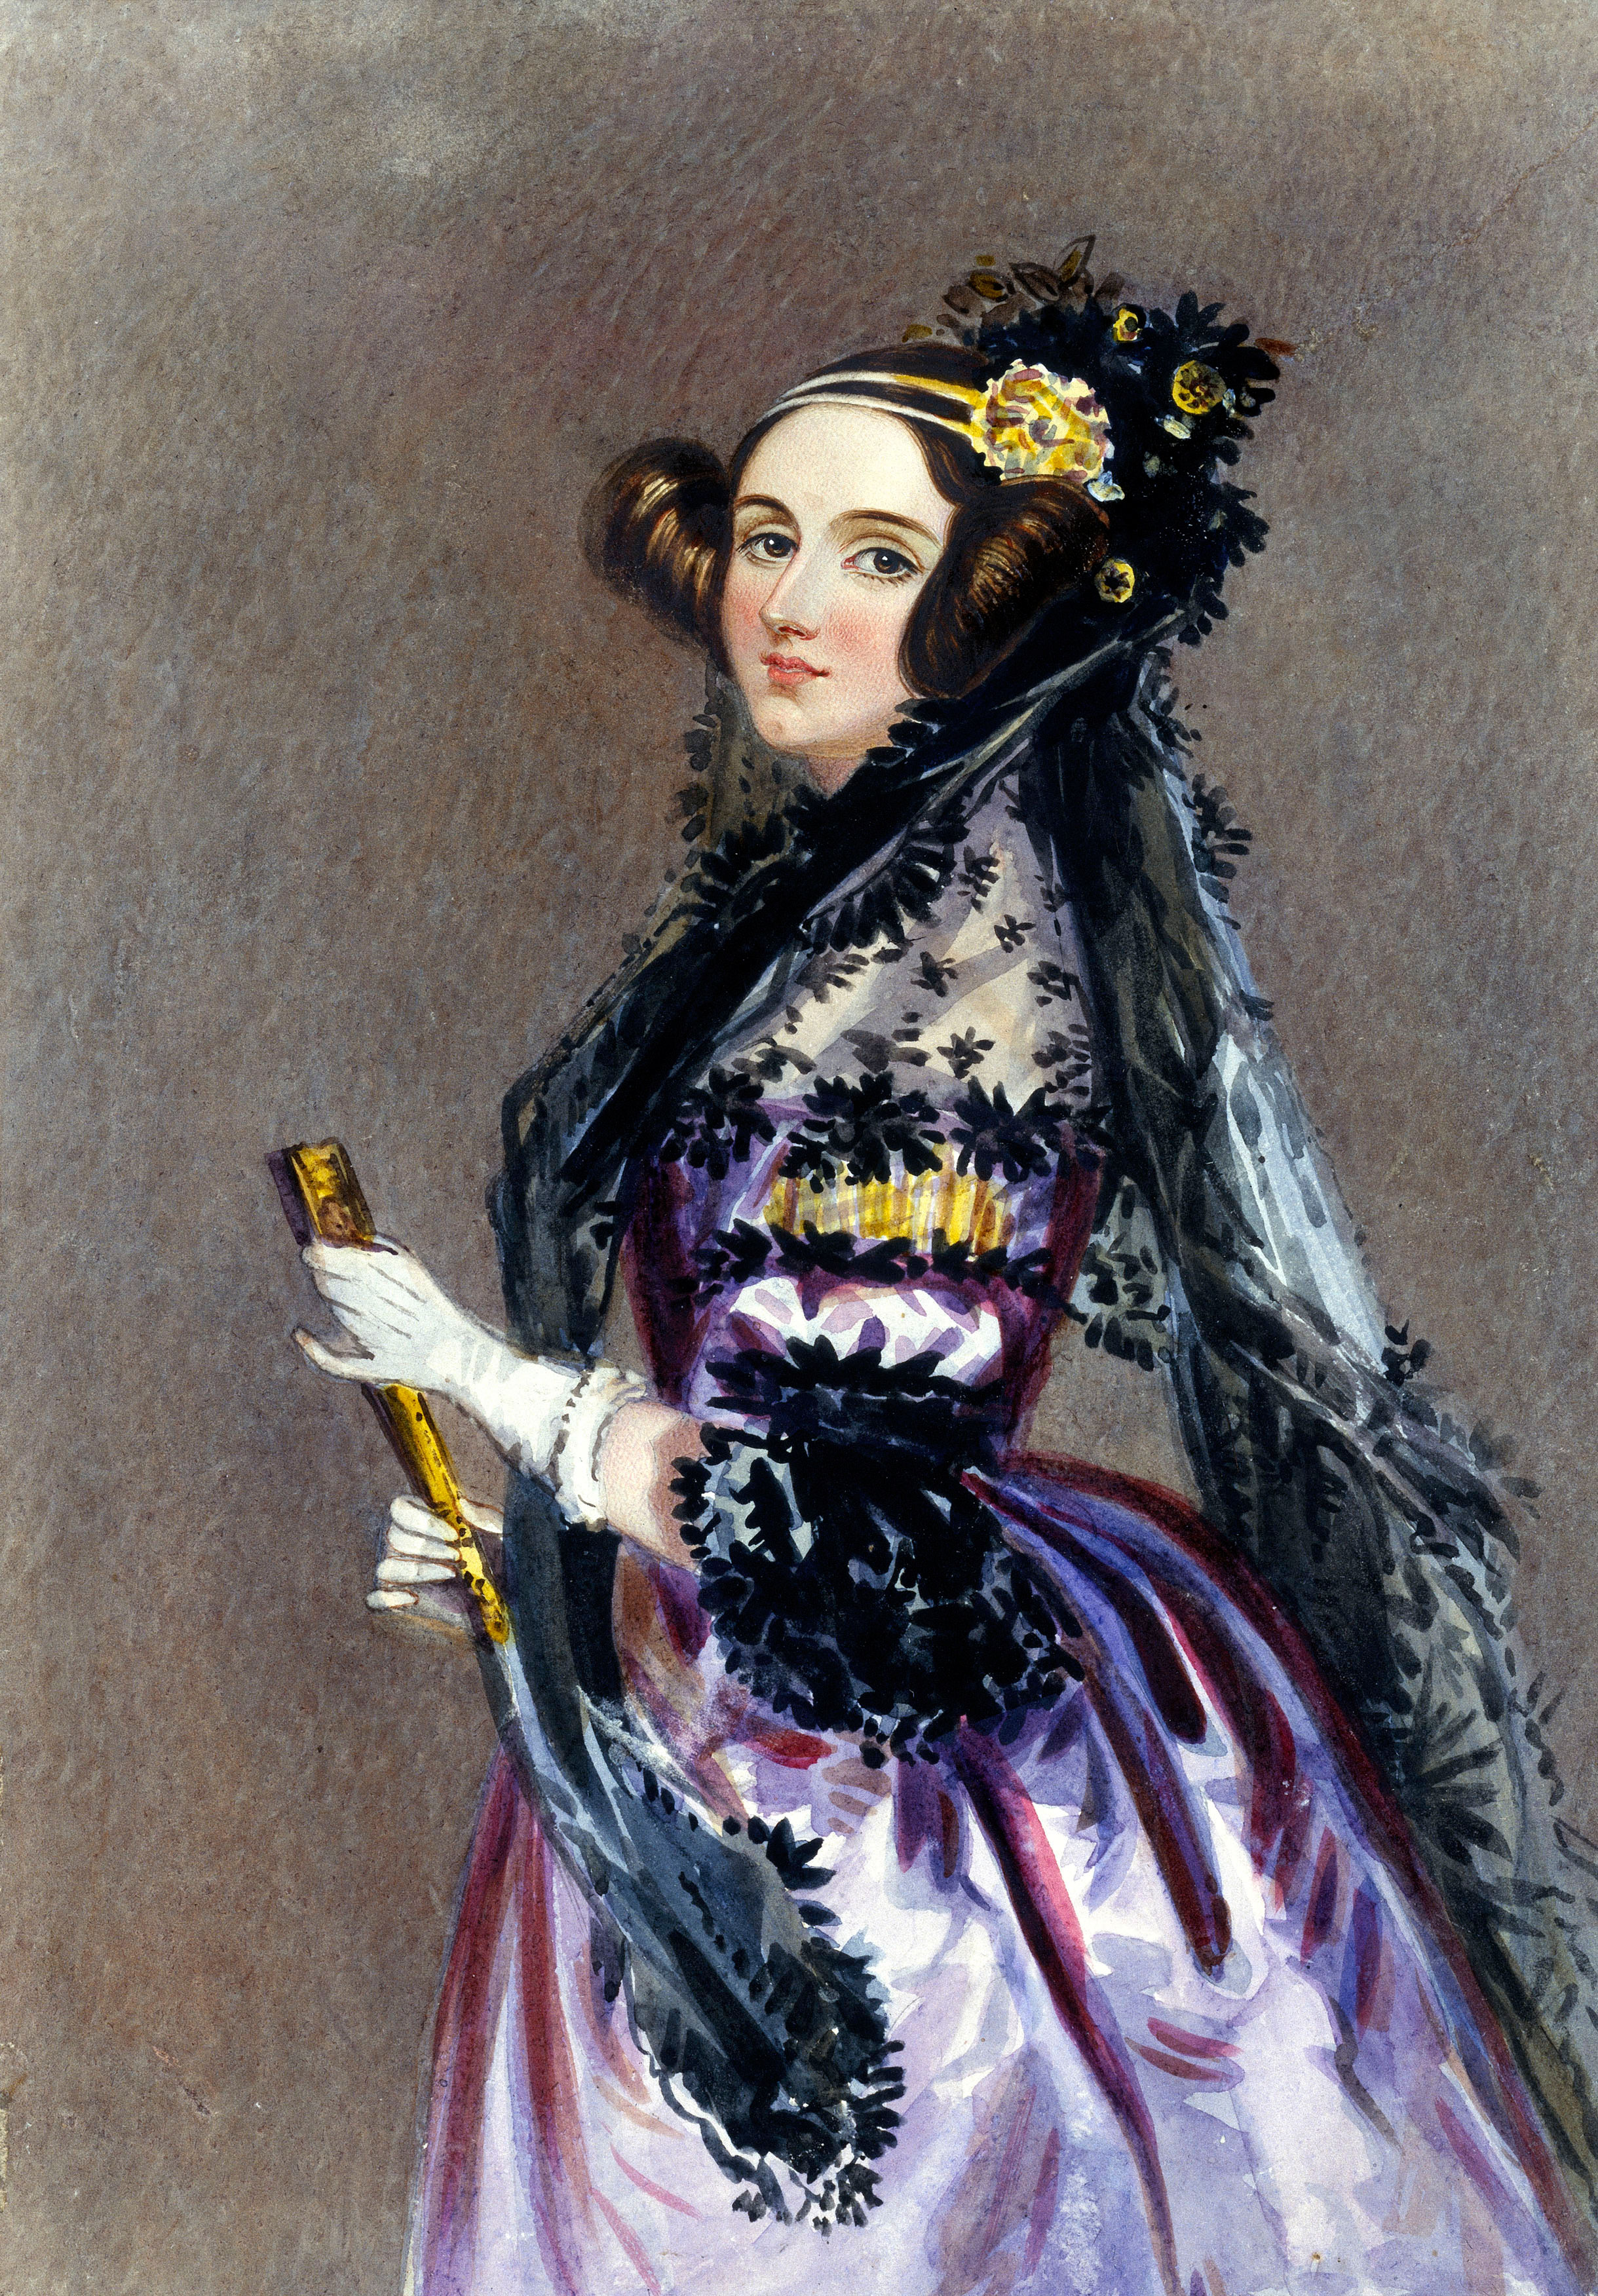
\includegraphics[width = 5 cm]{pic/lovelace} % Include a department/university logo - this will require the graphicx package
\end{center}



\begin{bottompar}
% ---- Professor -----
\begin{flushleft} \large
Dr. \textsc{Catasta} Michele\\
Distributed Information Systems Laboratory (LSIR) \\
\mail{michele.catasta@epfl.ch} \\ 
\end{flushleft}

% ---- date
{\large June 10, 2016}\\[1cm] % Date, change the \today to a set date if you want to be precise

\end{bottompar}
 
%%----------------------------------------------------------------------------------------
%% AUTHOR SECTION
%%----------------------------------------------------------------------------------------

%
%
%
%
%
%\begin{minipage}[t]{0.4\textwidth}
%
%\end{minipage}
%~
%\begin{minipage}[t]{0.55\textwidth}
%%\begin{flushright} \large
%%\emph{Assistant:} \\
%%\textsc{Voirol} Nicolas \\
%%PhD student\\
%%\mail{nicolas.voirol@epfl.ch} \\ [0.4cm]
%%
%%\emph{Supervisor:} \\
%%\textsc{Kuncak} Viktor\\  % Supervisor's Name
%%Professor\\
%%LARA - Laboratory for Automated Reasoning and Analysis\\
%%\mail{viktor.kuncak@epfl.ch}
%%\end{flushright}
%\end{minipage}\\[2cm]

% If you don't want a supervisor, uncomment the two lines below and remove the section above
%\Large \emph{Author:}\\
%John \textsc{Smith}\\[3cm] % Your name

%----------------------------------------------------------------------------------------
% LOGO SECTION
%----------------------------------------------------------------------------------------



%----------------------------------------------------------------------------------------
% DATE SECTION
%----------------------------------------------------------------------------------------

%{\Large \today}\\[1cm] % Date, change the \today to a set date if you want to be precise


%
%\begin{center}
%\abstract{\large Experiment various methods to compare functional trees between them. Given a function, use these algorithms to find the most similar tree contained in a corpus of functions. Try to suggest an autocompletion for a "hole" in a tree, based on this corpus.}
%\end{center} 
 %{\Large IDQ CONFIDENTIAL}
%----------------------------------------------------------------------------------------
\vfill % Fill the rest of the page with whitespace

\end{center}
\end{titlepage}



\pagestyle{fancy}
% ================ Table of content ==============
\newpage
\tableofcontents 

\baselineskip=16pt
%\parindent=15pt
%\parskip=5pt

\newpage




% ================ Introduction ==============
\section{Introduction}

\subsection{General information about the course}

This course covers multiple topics in the data science field such as \textbf{Data Wrangling}, {\bf Data Management}, {\bf Data Mining}, {\bf Machine Learning}, {\bf Visualization}, {\bf Statistics} and {\bf Story telling}. It's about {\bf breadth}, not depth. Indeed, Data science is evolving really quickly, hence learning in depth a specific tool won't pay off. 

\subsection{Data Science}

When we talk about Data Science, we often use the term Big Data as the enormous amount of data that exist in the world. But Big Data is not only about collecting huge amount of data. It is challenging but not enough. The real value comes from the insights. The {\it internet} companies (Google, Facebook, etc.) 
understood this many years ago.
\\ \\
An accurate definition of Data Analysis is given by Wikipedia:
\begin{framed}
{\it {\bf Analysis of data} is a process of {\bf inspecting}, {\bf cleaning}, {\bf transforming}, and {\bf modeling data} with the goal of {\bf discovering useful information}, suggesting conclusions, and supporting decision-making.
Data analysis has multiple facets and approaches, encompassing diverse techniques under a variety of names, {\bf in different business}, science, and social science {\bf domains}.}
\signed{\href{https://en.wikipedia.org/wiki/Data\_analysis}{Wikipedia - Data Analysis}}
\end{framed}

Therefore, a Data Scientist has to master different kind of skills such as {\bf Mathematics} (for the Statistics), {\bf Programming} and the {\bf Domain Expertise}. Drew Conway's Venn diagram, Figure \ref{img:venn}, shows the different combination man can obtain with these three skills.

\begin{figure}[H]
 \centering
 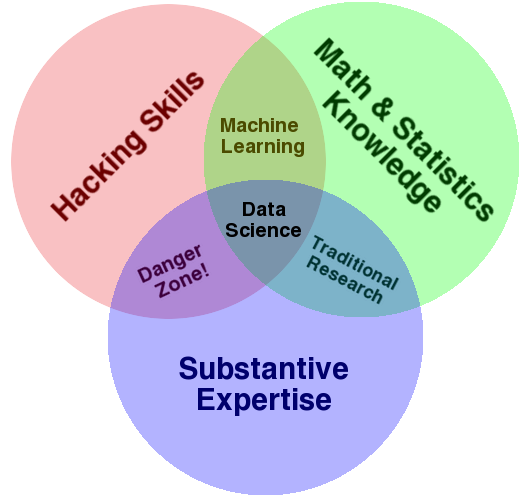
\includegraphics[width=7cm]{./pic/Data_Science_VD.png}
 \caption{\label{img:venn} Venn Diagram describing the different combination of skills used by a Data Scientist (by Drew Conway)}
\end{figure}

\begin{figure}[H]
 \centering
 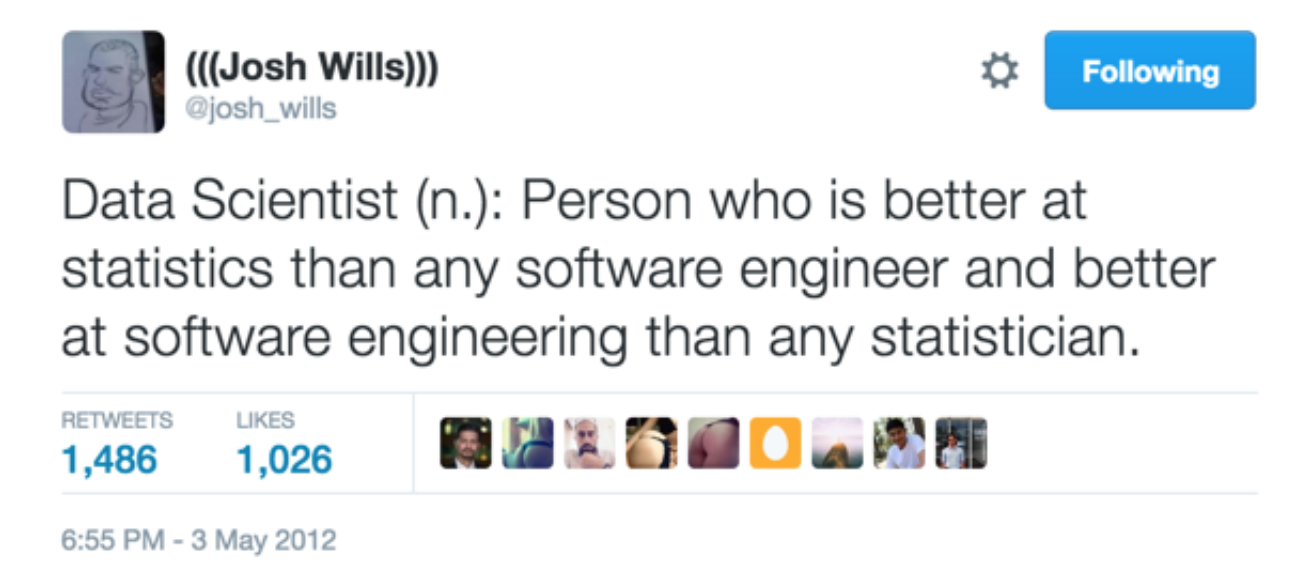
\includegraphics[width=10cm]{./pic/tweet_wills.png}
 \caption{\label{img:tweet_wills} A tweet from Josh Wills, Data Scientist at Slack.}
\end{figure}

{\bf A practical definition of Data Science} 

Data Science is about the whole processing pipeline to extract information out of data. As such, a Data Scientist {\bf understands and cares about the whole data pipeline}.

\begin{minipage}{0.5\textwidth}
\begin{figure}[H]
 \centering
 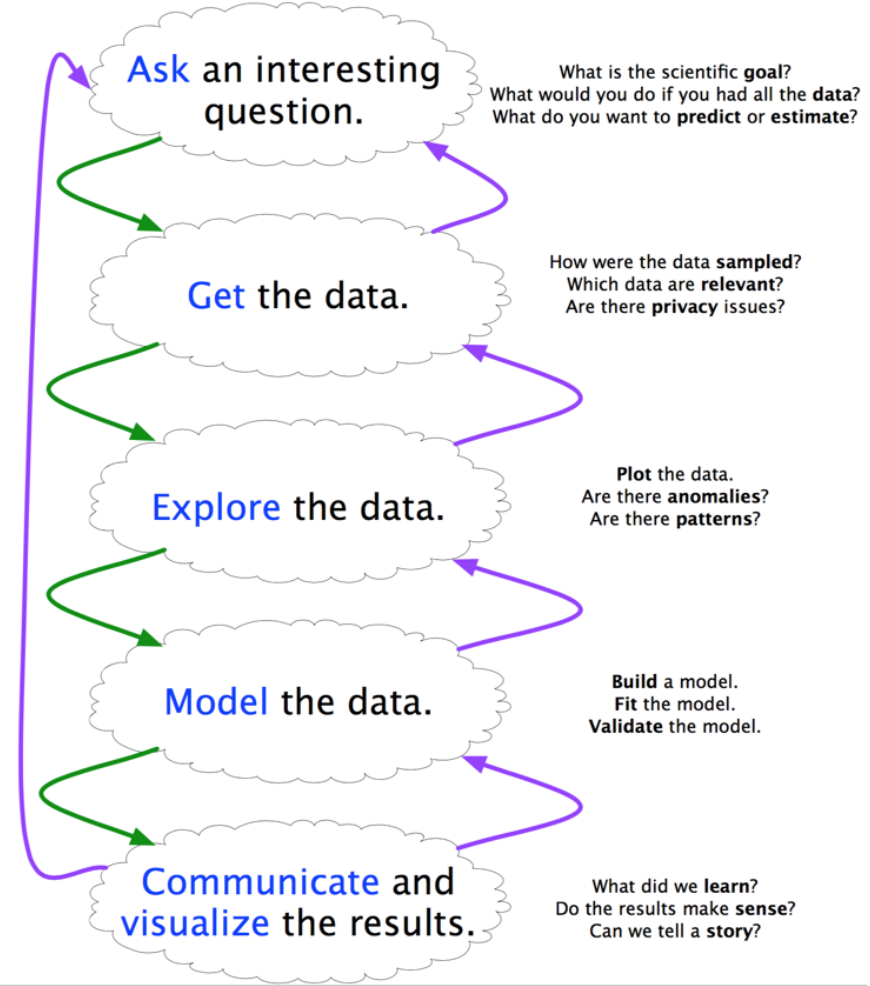
\includegraphics[width=8cm]{./pic/pipeline.png}
\end{figure}
\end{minipage} \hfill
\begin{minipage}{0.45\textwidth}
A {\bf data pipeline} consists of 3 steps:
\begin{enumerate}
 \item Preparing to run a model. \\
  {\it Gathering, cleaning, integrating, restructuring, transforming, loading, filtering, deleting, combining, merging, verifying, extracting, shaping}
 \item Running the model
 \item Communicating the results
\end{enumerate}
\vspace{0.5cm}
 A ``good'' Data Scientist will always go back and forth between the steps. The diagram on the left shows exactly what can happen. 
\end{minipage}
\\ \\
In this course, you will develop the following skills:
\begin{description}
 \item[data muning/scraping/sampling/cleaning] in order to get an informative, manageable data setlength
 \item[data storage and management] in order to be able to access data quickly and reliably during subsequent analysis
 \item[exploratory data analysis] to generate hypotheses and intuition about the data
 \item[prediction] based on statistical tools such as regression, classification, and clustering
 \item[communication of results] through visualization, stories and interpretable summaries
\end{description}


% ================ Definition ==============
% maybe to be moved at the end if it becomes a dictionnary
\section{Basic concepts}

A data science student is attended to understand the \textbf{Grammar of Data Science}. Having some backgrounds in SQL concepts is also a good thing because, as it is very common, people loves to make example with it. Here is a brief refresh of some definitions and concepts about data science.

\begin{itemize}
 \item {\bf Structured data} requires two key concepts:
 \begin{itemize}
  \item {\bf Data model} is a collection of concepts for describing data.
  \item {\bf Schema} is a description of a particular collection of data, using a given data model.
 \end{itemize}
 \item The {\bf Relational model} is on of the most common approach to manage data (SQL like) and can handle most of the data. A counter example is the facebook-like data which requires {\bf graph model}. This model is made of 2 parts:
 \begin{itemize}
  \item The {\bf Schema}. \\ For example, \verb+Students(sid: string, name:string, age:integer)+
  \item The {\bf Instance}, {\it i.e.} the data at a given time. \\
  Definitons:
  \begin{itemize}
   \item {\bf Cardinality} is the number of rows. (Number of items)
   \item {\bf Degree} or {\bf Arity} is the number of fields. (Number of attributes)
  \end{itemize}
 \end{itemize}
 \item Definitions of some ``Database'' terms:
 \begin{itemize}
  \item A {\bf JOIN} is a mean to combine tables based on shared attributes (most of the time some \textbf{IDs}). Despite its apparent simplicity beware of the many ways to compute a JOIN and check what is the default JOIN of a language before using it. The FIG \ref{join_SQL} summarises these possibilities.
  \item \textbf{Aggregation}, \textbf{reduction}, and {\bf groupby} are the action of reducing data with a common opperation (\textbf{sum}, \textbf{count}, \textbf{average}, ...) to summarise them. 
 \end{itemize}
 \item Definitions of some ``Pandas'' terms:
 \begin{itemize}
  \item {\bf Series} are a name, ordered dictionary
  \begin{itemize}
   \item keys are indexes
   \item built on \textbf{numpy.ndarray} (so values can be any Numpy data type)
  \end{itemize}  
  \item \textbf{DataFrame} is a table with named column
  \begin{itemize}
   \item the columns are series
   \item it is indeed a dictionary with (columnName $\rightarrow$ series)
  \end{itemize}  
 \end{itemize}
\end{itemize}

\begin{figure}%---------------FIG--------------
 \centering
 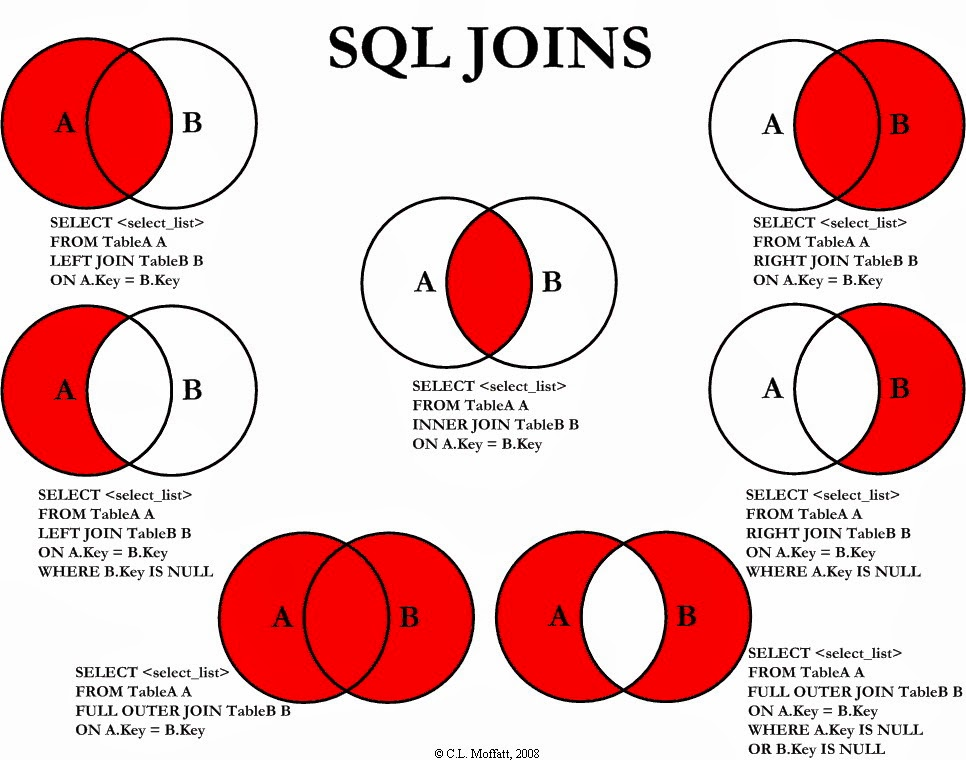
\includegraphics[width=12cm]{./pic/SQL_joins}
 \caption{\label{join_SQL} Different ways to join two tables and the related SQL command.}
\end{figure}


\subsection{Panda vs SQL}

Panda is built to allow easy and fast \textbf{data exploration} and not to be a database manager, as SQL is. Thus there are benefits and drawbacks of using it.


\begin{center} %---------------TAB--------------
\begin{tabular} {| l | l |}
\hline
\bf Pros & \bf Cons \\ \hline
Lightweight \& fast & Tables stored directly in memory \\
Great expressivness (combine SQL + Python) & No post-load indexing functionality\\
Easy plot for data visualization (eg Matplotlib) & No transactions, journalings\\ 
& Large, complex joins are slower \\ \hline
\end{tabular}
\end{center}

\subsection{OnLine Analytical Processing (OLAP cubes)}

OLAP tools enable users to analyze multidimensional data interactively from multiple perspectives. Conceptually, it is like an n-dimensional spreadsheet (a cube) on which we can apply various opperations to take decisions.

OLAP cubes are an other way to see data table and are contructed based on them, as shows FIG \ref{OLAP_cubes}.

\begin{figure}[H]%---------------FIG--------------
 \centering
 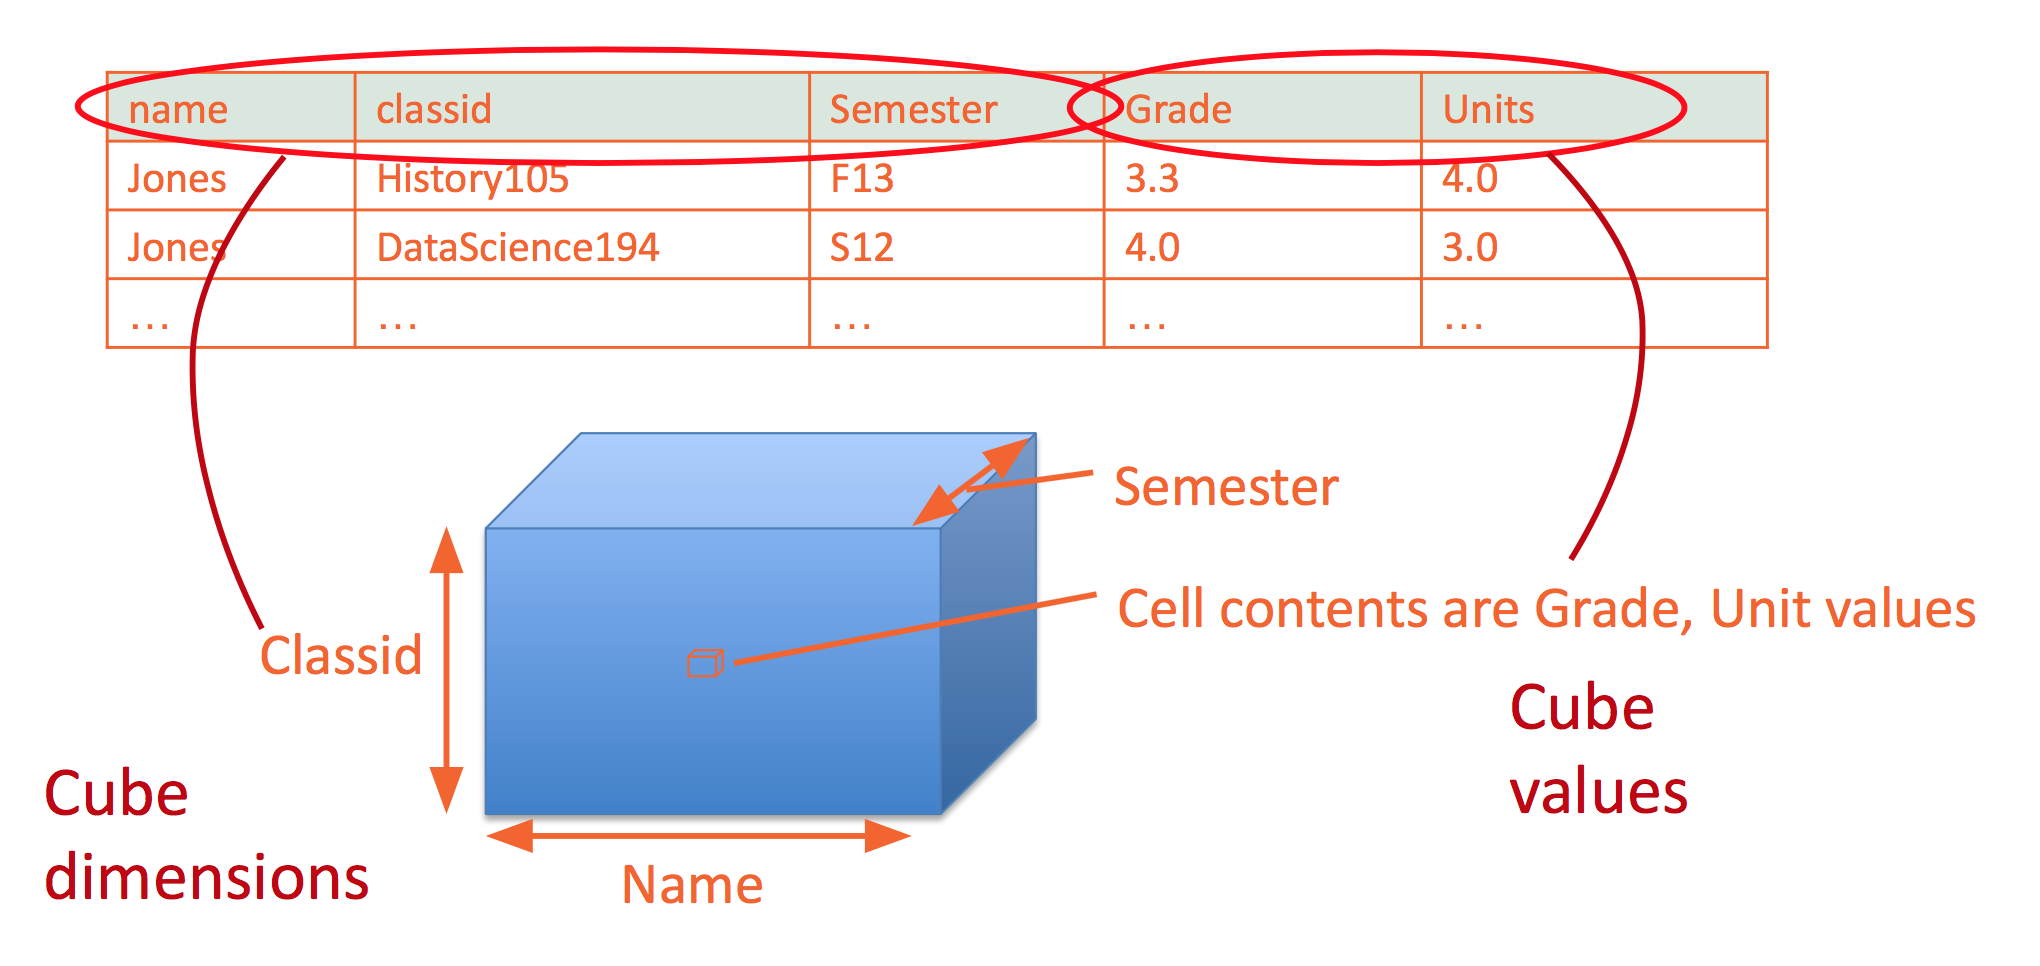
\includegraphics[width=12cm]{./pic/OLAP_cube}
 \caption{\label{OLAP_cubes} Construction of an OLAP cube from a table.}
\end{figure}

Operations on OLAP cubes are the following and are illustrated on FIG \ref{OLAP_operations}
\begin{itemize}
	\item \textbf{Slicing} fixes one or more variable
	\item \textbf{Dicing} selects a range of one or more variable
	\item \textbf{Driling up/down} changes levels of a hierarchically-indexed variable, ie "zoom" on a variable and see the sub-categories it contains.
	\item \textbf{Pivoting} change the point of view of the cube. Swap an aggregated variable an a detailed one.
\end{itemize}

\begin{figure} [h] %----------- SubGraph ---------------------
\centerline{
\subfigure[Slincing\label{olap_slicing}] {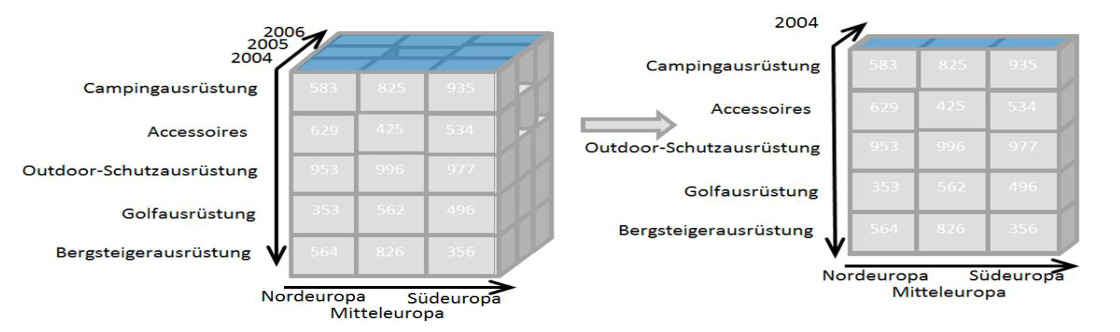
\includegraphics[width=7cm]{pic/Slicing} }
\subfigure[Dicing\label{olap_dicing}] {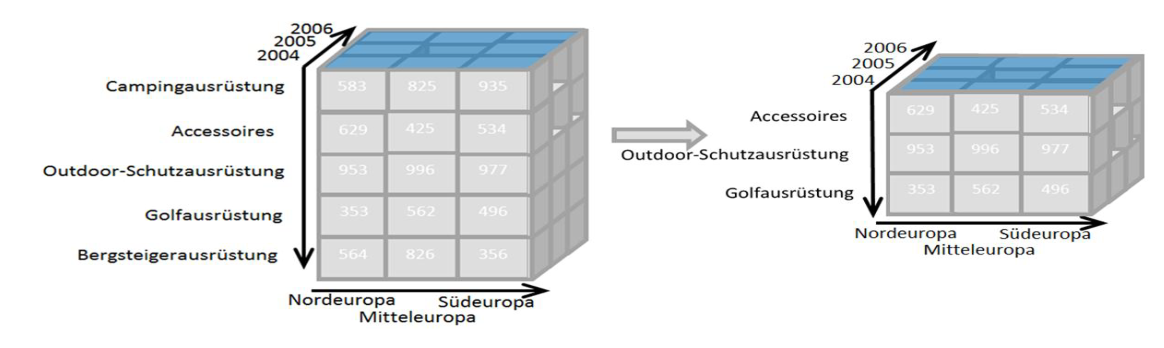
\includegraphics[width=7cm]{pic/Dicing} } 
}
\centerline{
\subfigure[Driling up/down\label{olap_driling}] {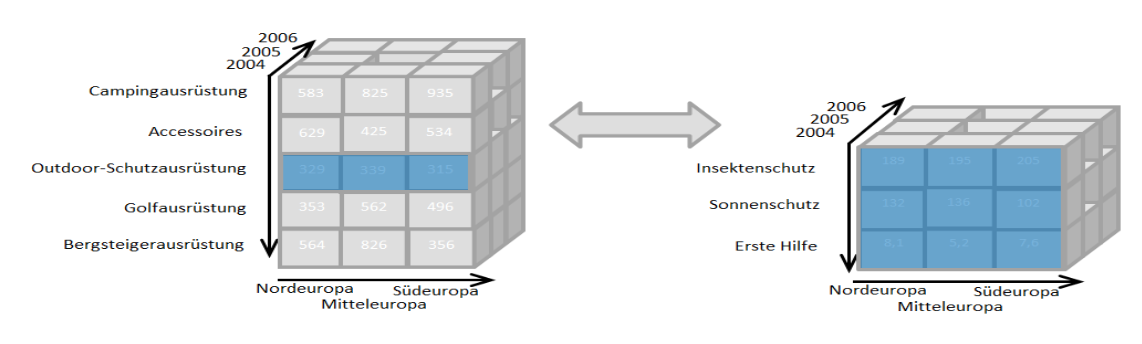
\includegraphics[width=7cm]{pic/Drilling_up_down} }
\subfigure[Pivoting\label{olap_pivoting}] {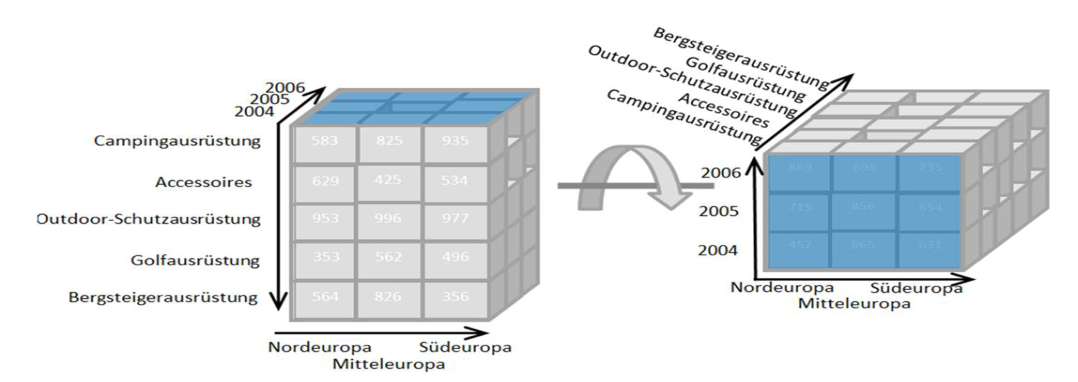
\includegraphics[width=7cm]{pic/Pivoting} } 
}
\caption{\label{OLAP_operations} Operations on OLAP cubes} 
\end{figure}

\begin{center} %---------------TAB--------------
\begin{tabular} {| l | l |}
\hline
\bf Pros & \bf Cons \\ \hline
& \\
\parbox[t][][t]{7cm}{The main adventage of OLAP cubes is that their are \textbf{conceptualy simpler} to understand by a non-scientist person, eg a business man who have to take day-to-day decisions based on company's data. Aggregations are limited but cover the main common cases that we can encounter.
}&
\parbox[t][][t]{7cm}{Because of the "on-line" behaviour of this approach, all type of aggregation must be pre-calculated amoung all combination of axis which is very \textbf{expensive in memory and in time} (when updating the data)}\\
& \\
\hline
\end{tabular}
\end{center}

% ================ Data Wrangling ==============
\section{Data Wrangling}

\begin{figure}[H]%---------------FIG--------------
 \centering
 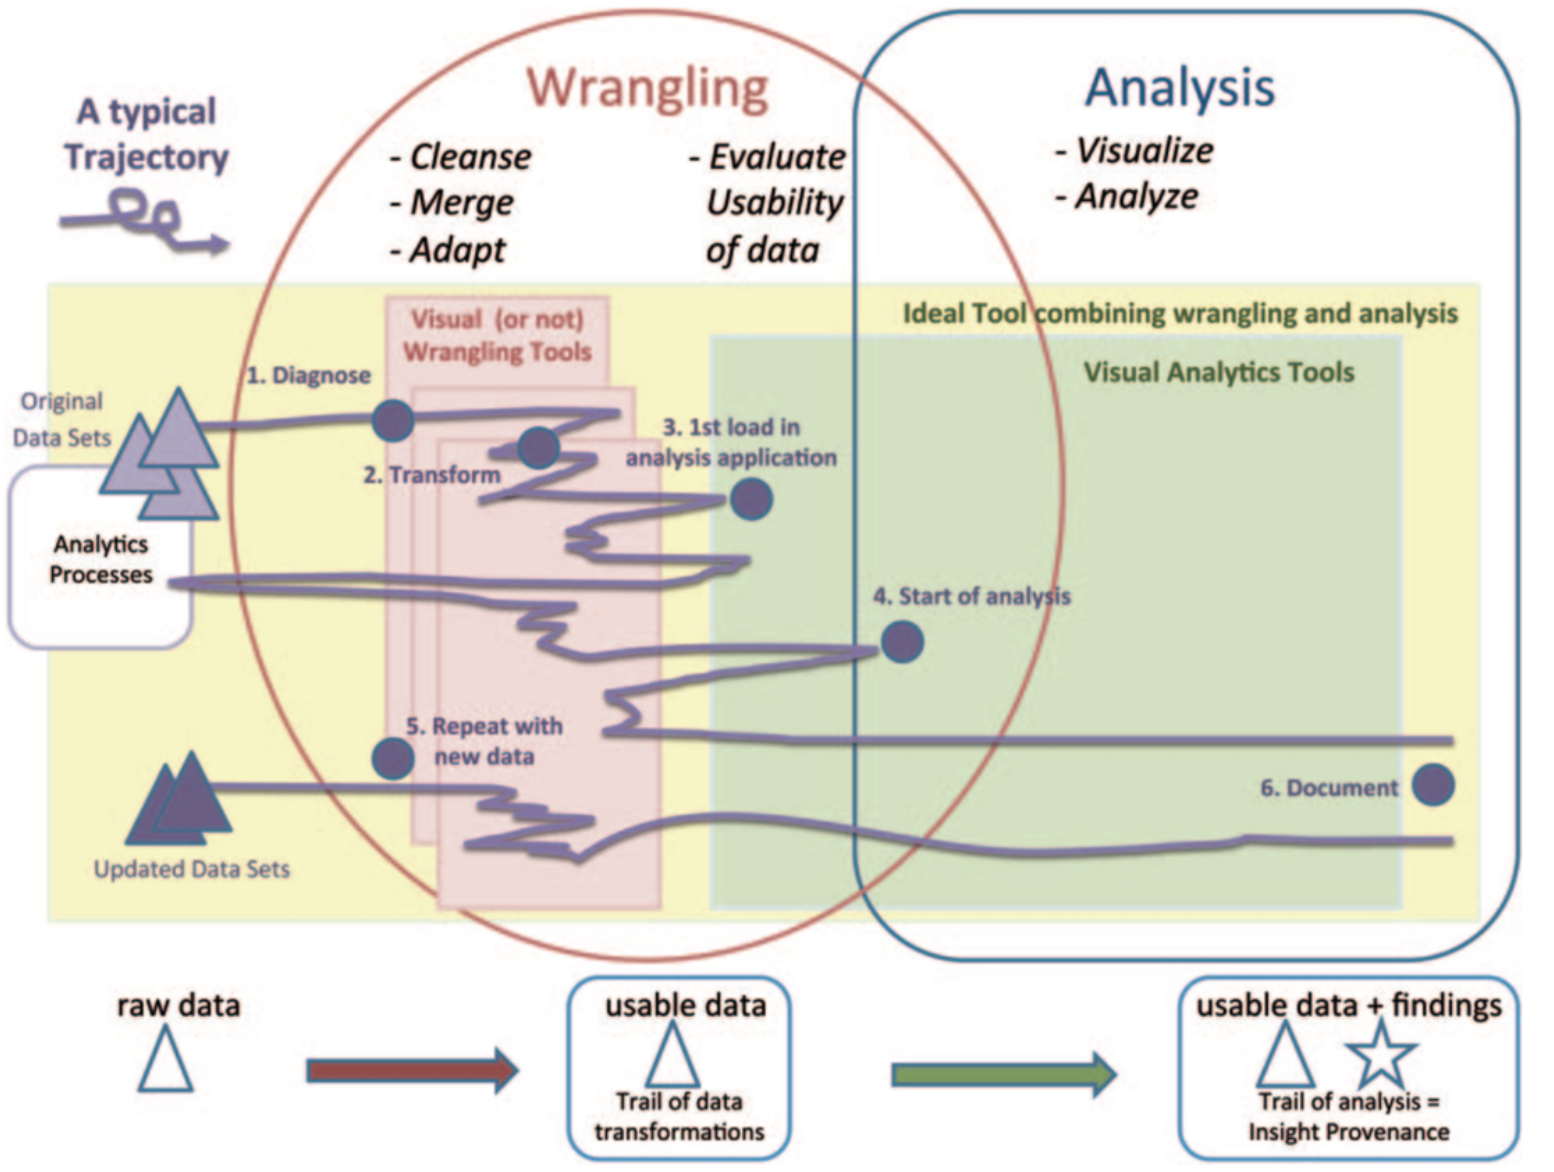
\includegraphics[width=12cm]{./pic/path_data_wrangling}
 \caption{\label{path_data_wrangling}Things do not always happen as expected...}
\end{figure}

Before any analysis, data need to be transformed from "dirty" to clean and processable data. 

Data comes from different sources (excel or SQL?), sometime collected through different methods over time, with different conventions (space or NaN?), etc ... Data wrangling's goal is to \textbf{extract and standardize these raw data}. The best way to do it is to \textbf{combine automation with visualizations} in order to find outliers. 

Data's problem can come from (non-exhaustive): 
\begin{itemize}
  \item Missing data
  \item Incorrect data
  \item Inconsistent representations of the same data
  \item Non-standardized data (centimeter or inches? farenheit or celsuis ?)
  \item Duplicated data
\end{itemize}

About 75\% of theses problem will need \textbf{human intervention} to be corrected (by the data-scientist or by crowdsourcing).

Even if it seems really dirty, \textbf{beware not to over-sanitize the data!}. Applying what we can call "defensive programming" is not a good idea because we risk to lose any interesting data, keeping only the ones that fit perfectly in our model.

\subsection{Diagnosis of the data}

One of the most important aspect of Data Wrangling is to {\bf understand} the data and to {\bf find possible problems}. In order to ``diagnose'' the data, two tools can be used:
\begin{itemize}
 \item {\bf Visualization} (A {\it toughtful} visualization will always help)
 \item {\bf Basic Statistics} 
\end{itemize}

Matrix visualizations of the facebook graph is shown in Figure \ref{pic:fb}. The Relational visualization, Figure \ref{pic:fb1}, does not show any particular problem in the data. But the Time dependant visualization, Figure \ref{pic:fb2}, shows that the Facebook API reached its limit while collecting data.

\begin{figure} [h] %----------- SubGraph ---------------------
\centerline{
\subfigure[Relational visualization \label{pic:fb1}] {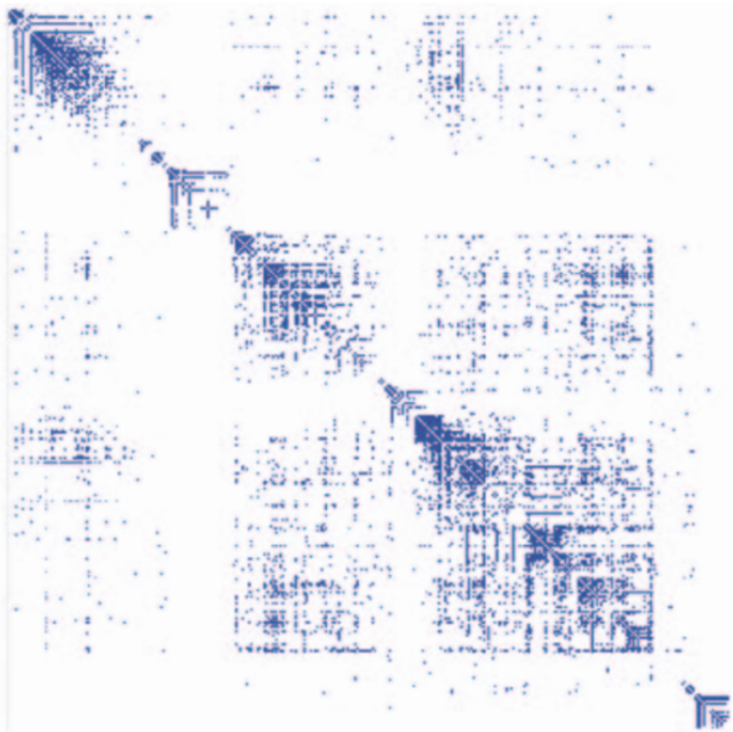
\includegraphics[width=7cm]{pic/fb1} }
\subfigure[Time dependant visualization\label{pic:fb2}] {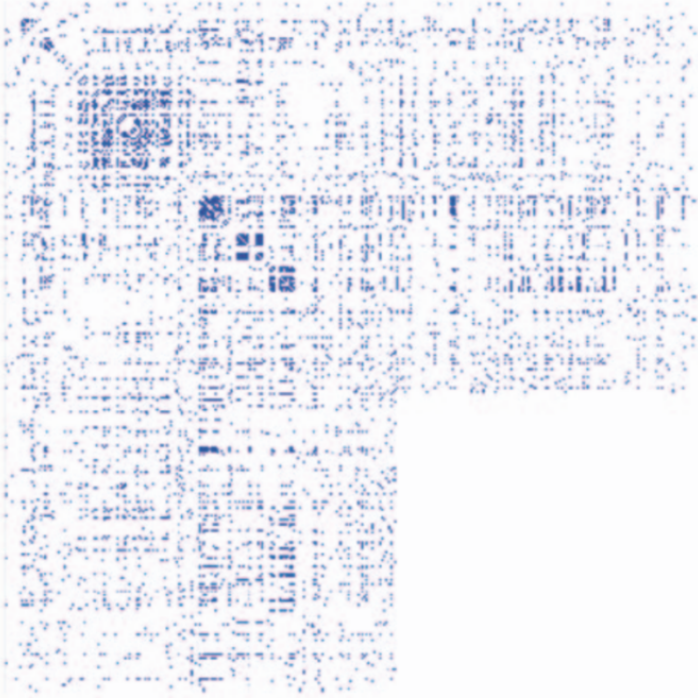
\includegraphics[width=7cm]{pic/fb2} } 
}
\caption{\label{pic:fb} Matrix visualization of the facebook graph.} 
\end{figure}


\subsection{Dealing with missing values}

Values can often miss from the data we have, because of various events (war, fire, ...). We must detect and correct these values with different method according with the domain we are working in.

Whatever the method used, it's good to keep track of these changes to know which are original data and which are modified ones.

\begin{itemize}
  \item Set values to zero FIG \ref{miss_val}(a)
  \item Interpolate based on existing data FIG \ref{miss_val}(b)
  \item Omit missing data FIG \ref{miss_val}(c)
  \item Interpolation with track kept \ref{miss_val}(d)
\end{itemize}

\begin{figure}[H]%---------------FIG--------------
 \centering
 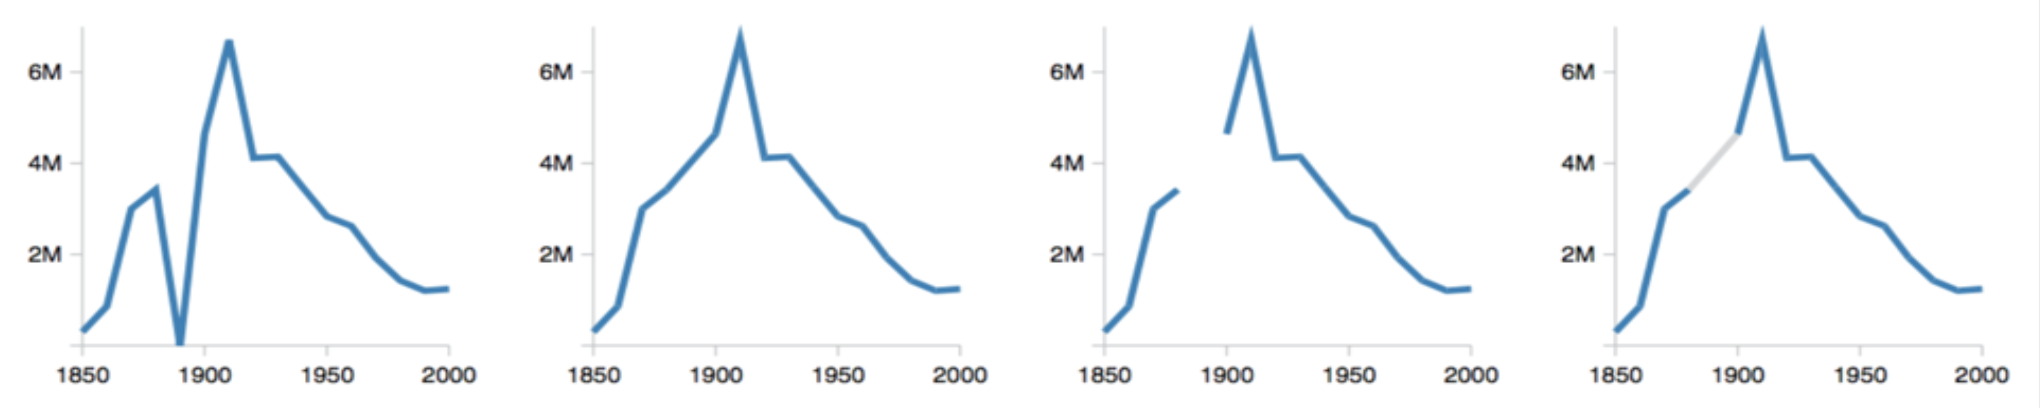
\includegraphics[width=15cm]{./pic/missing_values}
 \caption{\label{miss_val}To deal with missing values.}
\end{figure}

\subsection{General procedure}

Once the data are well wrangled and before trying to analyse them we must take care of two more steps:

\begin{enumerate}
  \item \textbf{Deal with uncertain data} (can arise from measurement errors, wrong sampling strategies, etc.)
  \item \textbf{Parse/trasform data} (with aggregation and reduction techniques) to obtain meaningful records
\end{enumerate}
 
It's always ideal to have the code and/or the documentation about the dataset you are analyzing (provenance).
 
% ================ Data Variety ==============
\section{Data Variety}

The ``3 Vs'' of Big Data: {\it Volume}, {\it Velocity} and {\it Variety}. In this course, we don't address the {\it Volume} and {\it Velocity} parts (A course on Database does). Since there is a lot of variety in the data, we need to prepare the data. This flow is called {\bf ETL}:
\begin{itemize}
 \item {\bf Extract} from the {\it source(s)}.
 \item {\bf Transform} data at the source, sink, or in a {\it staging area}.
 \item {\bf Load} data into the {\it sink}.  
\end{itemize}
This variety of the data comes, in a first place, from the many different sources from which we extract them: {\it files, databases, logs, ... } Each of these sources uses (or not!) its proper convention and can contains structured (DB), semi-structured (logs) or unstructured (web page) data. 

\subsection{Role of Schema}
The {\bf Schema}, which specifies the {\it structure} and {\it types} of data repository, is changing. Traditional databases are {\bf schema-on-write}, {\it i.e.} you cannot load data into a table without a schema. But new data stores (NoSQL for example) are {\bf schema-on-read} or {\bf schemaless}. 

\begin{itemize}
	\item {\bf Schema-on-write} is typically SQL, where we must create a table before inserting data in our system. Data must scale the defined schema and this is both the strength and weakness of the system. Strength because the data is perfectly oriented and respect the constraints we establish. Weakness because schemas are always subjective in some ways and data (which are perfectly corrects) may not fit with it. 
	\item {\bf Schema-on-read} is for instance XML, where you create the schema according with the data you read.
	\item Youtube and Google Cache where the first {\bf schemaless} data system. Without schema, everything is simply stored as a string and we need a parser to return a typed data.
\end{itemize}

\subsection{Examples of data}

\subsubsection{XML and DOM}

The XML data are used mostly with HTML and specifies the data structure. An XML schema can be applied to interpret the XML data and specifies the {\bf data types}. Figure \ref{pic:xml} shows the XML data \ref{pic:xml_data} and the schema \ref{pic:xml_schema} used to parse and type the data.

\begin{figure} [h] %----------- SubGraph ---------------------
\centerline{
\subfigure[XML data \label{pic:xml_data}] {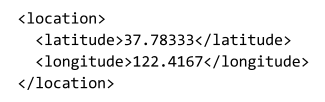
\includegraphics[width=5cm]{pic/xml_data} }
\subfigure[XML schema\label{pic:xml_schema}] {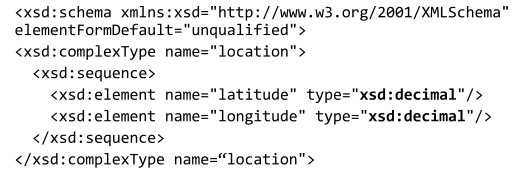
\includegraphics[width=7cm]{pic/xml_schema} } 
}
\caption{\label{pic:xml} Example of XML.} 
\end{figure}

The XML is a text format that encodes {\bf DOM} (Document-Object Models). It's a data structure often used by Web pages. The DOM is tree-structured. An example of a DOM is given in Figure \ref{pic:dom}.

\begin{figure}[H]%---------------FIG--------------
 \centering
 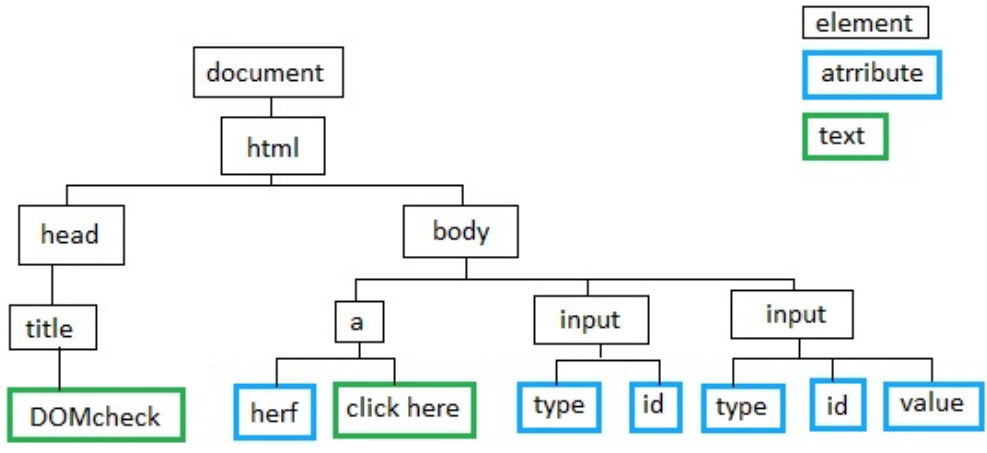
\includegraphics[width=10cm]{./pic/dom}
 \caption{\label{pic:dom} Example of a DOM tree for an HTML Web page.}
\end{figure}

THe XML schema allows a database to interpret the data when running queries. It can do arithmetic or range queries on numerical values, for example.

\subsubsection{JSON}

{\bf JSON} stands for Javascript Object Notation. It's a schemaless data (schema support was added later). An example of JSON data is shown in Figure \ref{pic:json}

\begin{figure}[H]%---------------FIG--------------
 \centering
 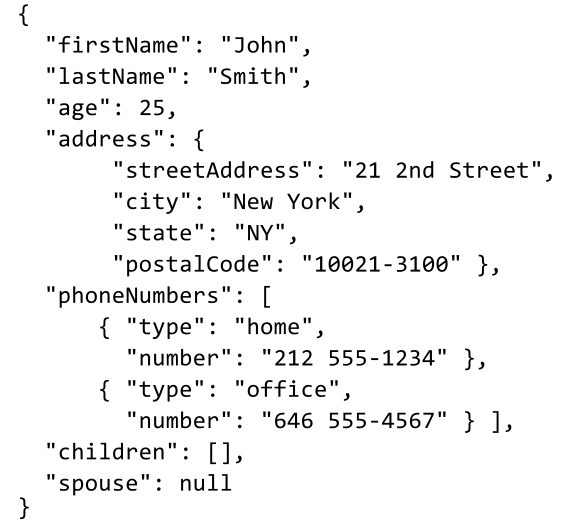
\includegraphics[width=8cm]{./pic/json}
 \caption{\label{pic:json} Example of a JSON data.}
\end{figure}

JSON is typically used to represent {\bf hierachical data structures} directly in the target language (Javascript or Java at the beginning). The transformation on the data are procedural in the target languages. It is often easier for some tasks, but it can be painful for some of them: for example schema changes.

\subsubsection{Tabular data}

A Tabular Data is simply data put into a table such as CSV or TSV. Definition of a table:
\begin{itemize}
 \item A {\bf table} is a collection of {\bf rows} and {\bf columns}.
 \item Each row has an {\bf index}.
 \item Each column has a {\bf name}.
 \item A {\bf cell} is specified by an (index, name) pair.
 \item A cell may or may not have a {\bf value}.
\end{itemize}

It's a very simple yet powerful data type. For example, the sensors usually output data in the form of time series, transformed into a tabular format. However, a system dealing with sensor data should:
\begin{itemize}
 \item support both long-term ({\bf trend}) and short-term ({\bf real-time}) queries
 \item have {\bf low latency} but also efficient. It should use {\bf real-time indexing} for longer-term queries.
 \item support triggers ({\bf alerts}) for a variety of conditions.
\end{itemize}
Therefore, the {\bf complexity of a data format} does not determine the {\bf complexity of the system required to properly handle it}.

\subsubsection{Log files}

The log files are simple text files giving information about process. The daemons, such as \verb+httpd+, \verb+mysqld+ or \verb+syslogd+, usually create logs. {\bf \verb+syslog+} was developed by Eric Allman. It's a way for devices to send event messages to a server that will log all the events. Splunk is a company that built a successfull business model around the syslog events.

\subsubsection{Binary formats}

They are often the key to performance because we {\bf avoid expensive parsing}. The modern formats even support nested structures, various level of schema enforcement, {\bf compression}, etc. Somes examples: Protocol Buffers (Google), Avro, Parquet, etc.

\subsection{Processing the data (JSON and XML)}

In order to process XML, we can use the DOM. It can also be used to process JSON data. The DOM is very easy to work with: all the data are directly accessible by links. The problem is that we {\bf might not care about most of the data} and if the data are big, they {\bf might not fit into the RAM}. In order to deal with these two problems, we can use a {\bf SAX} parser which is an event-driven parser. It will find all the {\bf open-close-tag events} in an XML document and will {bf do callbacks to user code}.

\begin{itemize}
\renewcommand{\labelitemi}{{\bf +}}
 \item User code can respond to only a subset of events corresponding to the tag it is interested in.
 \item User code can correctly compute aggregates from the data rather than create a record for each tag.
 \item User code can implement flexible error recovery strategies for ill-formed XML.
\renewcommand{\labelitemi}{{\bf --}}
 \item User code must implement a state machine to keep track of ``where it is'' in the DOM tree.
\end{itemize}

For JSON, most parsers construct the ``DOM'' directly. But there are a few SAX-style parsers: Jackson, JSON-simple, etc. Sometimes {\bf SAX-style is the way to handle ill-formed datasets}, an endless array of objects for example.

\subsection{HTML and Web Services}

\subsubsection{HTML}

Internet contains an ``enormous'' amount of data. Some crawlers such as Common Crawl dataset contains about 1.82 billions web pages (for 145 TB). We can use different tools to crawl data from the web. Examples for Python: Beautiful Soup, Requests, Scrapy, etc. 
\\\\
Most of the time, the Web pages are considered as unstructered data. But you can find some semi-structured data, {\it e.g.} Google WebTables. Some big ``internet'' companies (Google, Yahoo, Yandex and Microsoft) are sponsoring a project called {\bf schema.org} to create structured or semi-structured Web pages. A core vocabulary for the type of fields is given. schema.org is more and more used. It's also used by knowledge bases such as Google Knowledge Graph. {\bf WikiData} is a community project to create an open database of structured data taken from Wikipedia.

\subsubsection{Web Services}

Screen-scraping the content of a large website was possible before, but become more and more difficult nowadays. This is mainly due to the content "hidden" behind a form or an authentification. Take for example facebook without account, or the IS-academia course page if you do not select a semester. Therefore big companies are providing Web Service APIs\footnote{Application Program Interface: Set of subroutine definitions, protocols, and tools for building software and applications. In this particular case, the APIs are used to retrieve the data from the Web page, {\it e.g.} Facebook API to retrieve the contacts.} to retrieve data from their website. There are two kinds of Web Services:
\begin{itemize}
 \item The old way: XML-based RPC-style messages: SOAP
 \item The new way: REST-style stateless interactions, URLs encode state
\end{itemize}

\paragraph{RPC}

The SOAP RPC \footnote{SOAP = Simple Object Access Protocal, RPC = Remote Procedure Call} messages typically encode arguments that are presented to the calling profram as parameters and return values. HTTP POST/GET are used to communicate.
\begin{figure}[H]%---------------FIG--------------
 \centering
 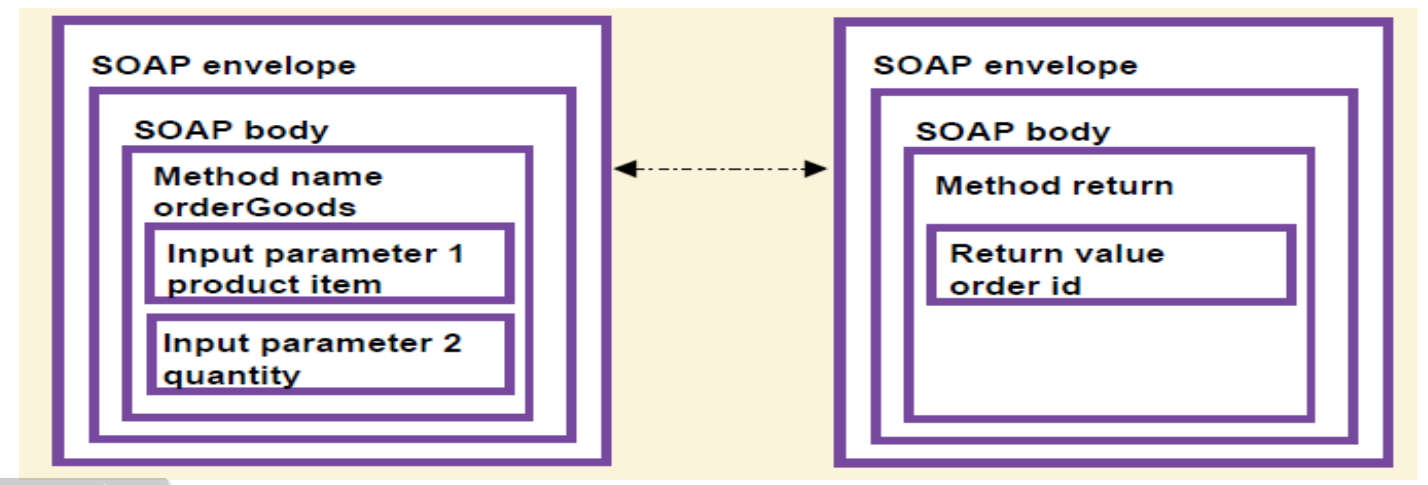
\includegraphics[width=13cm]{./pic/soap-rpc}
 \caption{\label{pic:soap-rpc} Example of a SOAP RPC exchange.}
\end{figure}
This kind of procedure (same for XML-RPC) requires a request-response cycle. This often leads to longer ``conversations''. The RPC-style is being quickly superseded by newer and more user-friendly technologies.\\\\
In {\bf RPC systems}, the design emphasis is on {\bf verbs}. It uses functions such as {\it getUser()}, {\it addUser()}, etc.


\paragraph{REST}

REST\footnote{REpresentation State Transfer} is a {\bf stateless} client/server protocol. The principles are:
\begin{enumerate}
 \item Each message in the protocol contains all the information needed by the receiver to understand and/or process it. This constraint attempts to {\it ``keep things simple''} and avoids needless complexity.
 \item Set of Uniquely Addressable Resources
 \begin{itemize}
  \item {\it ``Everything is a Resource''} in a RESTful system
  \item Requires universal syntax for resource identification, {\it e.g.} URI.
 \end{itemize}
 \item Set of Well-Defined Operations that can be applied to all resources
 \begin{itemize}
  \item In the context of HTTP (REST APIs), the primary methods are: \\
  {\bf POST}, {\bf GET}, {\bf PUT}, and {\bf DELETE} \\
  These are similar (but not exactly) to the database notion of CRUD (Create, Read, Update, and Delete)
 \end{itemize}
 \item The use of Hypermedia both for Application Information and State Transitions
 \begin{itemize}
  \item Resources are typically stored in a structured data format that supports hypermedia links, such as XHTML or JSON.
 \end{itemize}
\end{enumerate}
In {\bf REST systems}, the design emphasis is on {\bf nouns}. It uses the HTTP Protocols (POST, GET, PUT, and DELETE) a {\it User}, a {\it Location}, etc. 

% ================ Statistics ==============
\section{Statistics on the Data}

When we explore and analyze data, it would be great if we only had to look at some statistics numbers and make automatically a conclusion about them. Sadly, it's not the case. At all.
% ================  Famous mistakes ==============
\subsection{Examples of famous mistakes due to statistics}

%=================== Anscombe's quartet ===================
\subsubsection{Anscombe's quartet: Sensivity of outliers \& Robust statistics}

The FIG \ref{pic:anscombe} show four differents data distribution that present, despite all of that, the same means on $x$ and $y$, the same variance on $x$ and $y$, and, thus, the same linear regression function. This is due to the statistics used to define them. 

\begin{itemize}
    \item Min, Max, Mean, Standart Deviation (Std) and Range are sensitives to outliers and then are \textbf{not robust statistics}.
    \item Median, quartils, (and others) are not sensitives and then are said to be \textbf{robust statistics}. 
\end{itemize}



\begin{figure}[h]%---------------FIG--------------
 \centering
 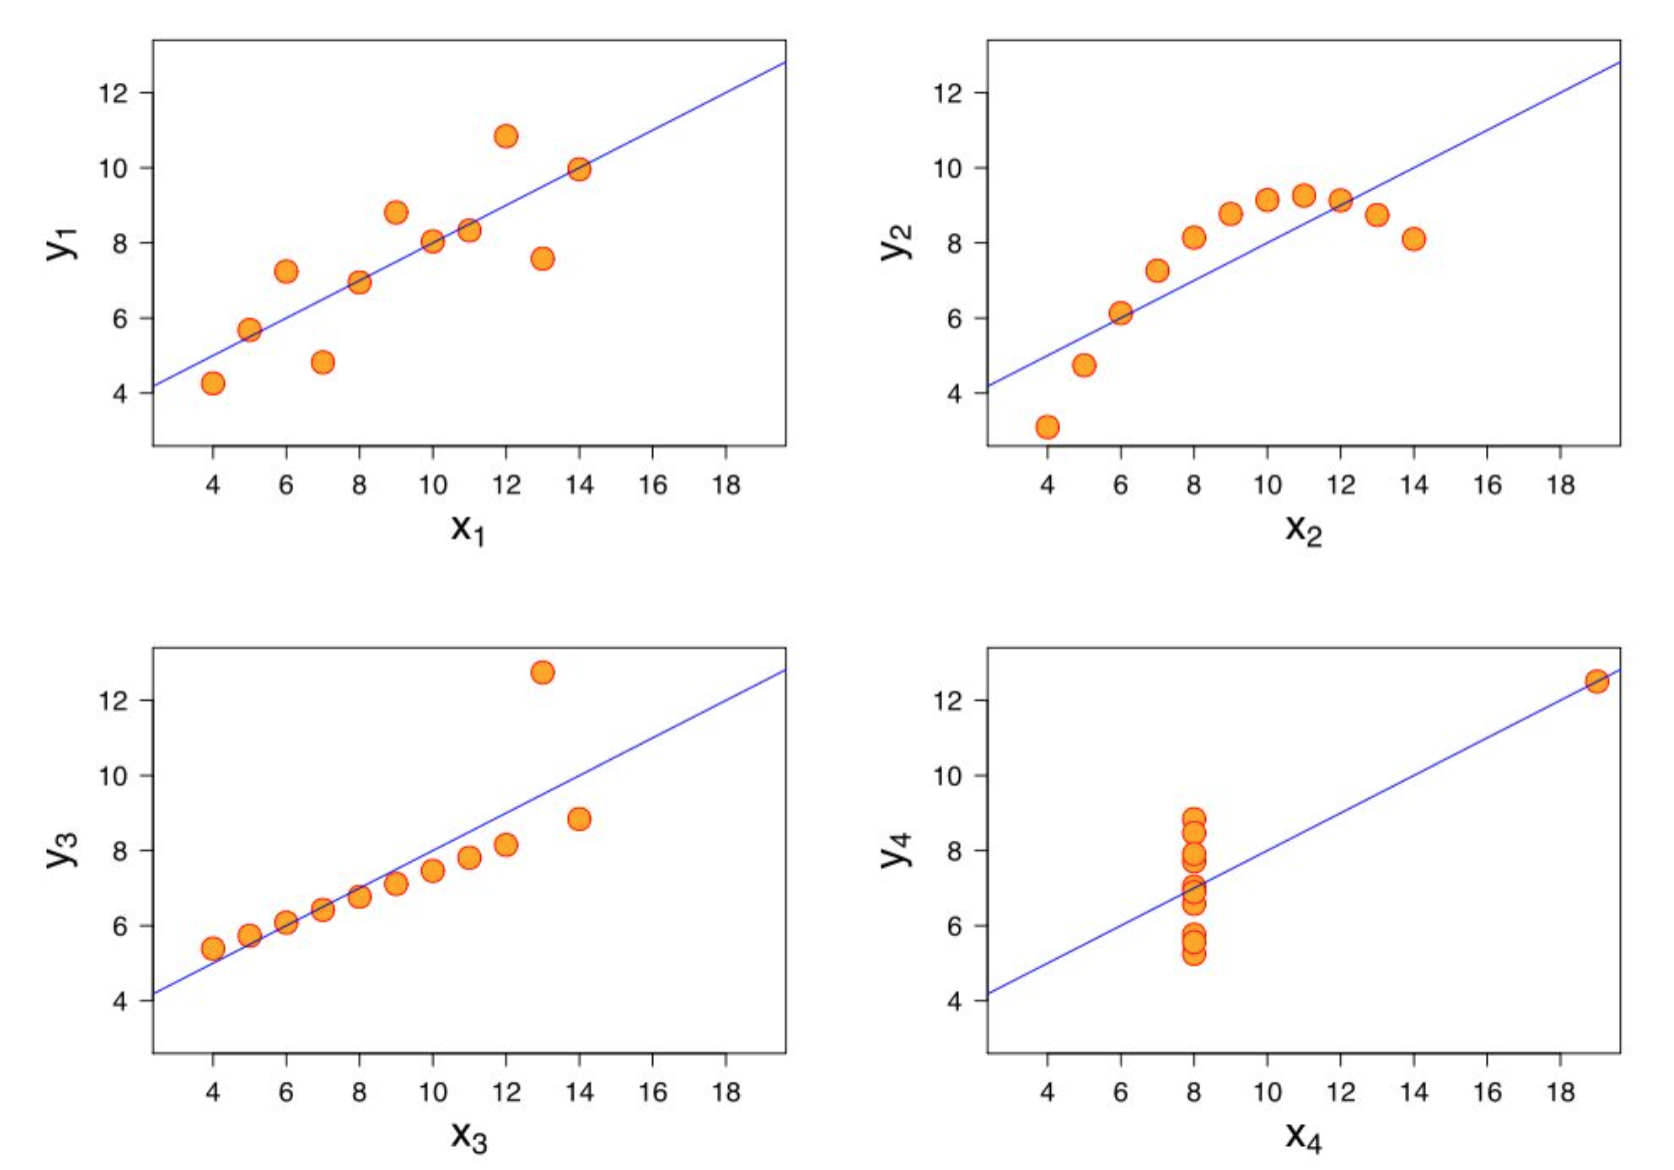
\includegraphics[width=10cm]{./pic/anscombe}
 \caption{\label{pic:anscombe} Anscombe's quartet}
\end{figure}

%================ Simpson paradox =================
\subsubsection{Simpson's paradox: aggregation of data}

\textbf{Certain tendencies can appear, disappear or even reverse themself when aggregating the data!} This was the case when media started blaming Berkey of being unfair with women applications (looking at left table of FIG \ref{pic:Berkley}). After further investigation (and de-aggregation of the data) it appeared that at the opposite... Berklay was unfair with men! (Right table of the same FIG).

This paradox comes from the fact that women (according with these tables) tended to apply for more competitiv departments, with lower rates of admission. \textbf{When aggregating the data, we lost this subtlety and then draw a wrong conclusion.} 

Simpson's paradox can appear in a lot of cases and can be very hard to detect. The \href{https://en.wikipedia.org/wiki/Simpsons_paradox}{wikipedia page of Simpson's paradox} describes a lot of examples and, for the ones interested, a great book relates lots of statistical errors that drove to miscarriages of justice: \href{https://books.google.ch/books/about/Math_on_Trial.html?id=PFAIb6FTgY4C&source=kp_cover&redir_esc=y&hl=fr}{Leila Schneps and Coralie Colmez, Math on Trial: How Numbers Get Used and Abused in the Courtroom} 

\begin{figure}[h]%---------------FIG--------------
 \centering
 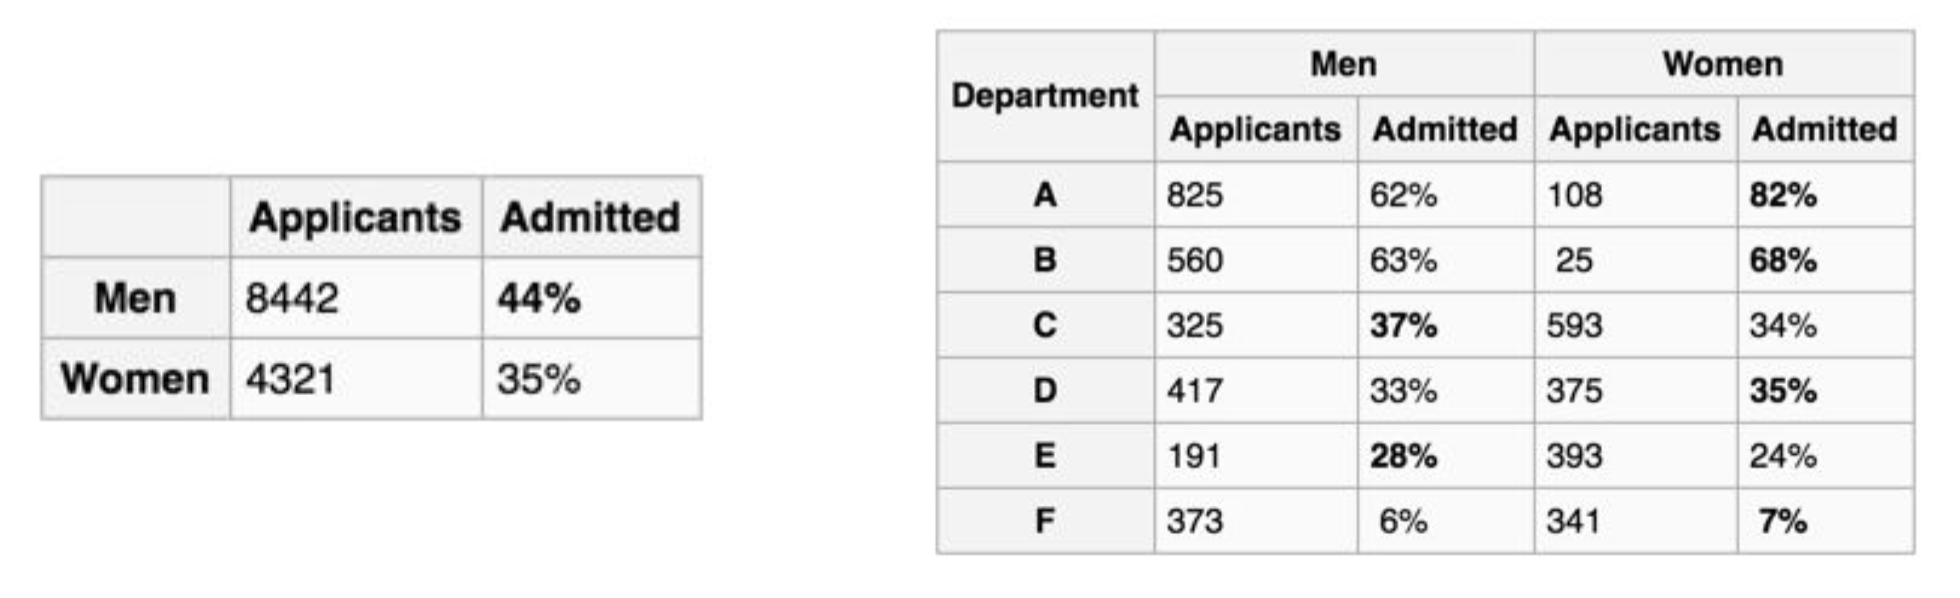
\includegraphics[width=10cm]{./pic/Berkley}
 \caption{\label{pic:Berkley}Berkley admission tables of 1973}
\end{figure}

% ================ Basic stats ==============
\subsection{Refresh of basic statistics concept}

\begin{itemize}
	\item {\bf Probabilities}: mathematical theory that describes uncertainty. \\
	\item {\bf Statistics}: Set of techniques for extracting useful info from data
\end{itemize}

\begin{framed}
{\it {\bf Probability and Statistics} are related areas of mathematics which concern themselves with analyzing the relative frequency of events. Still, there are fundamental differences in the way they see the world:\\
\textbf{Probability deals with predicting the likelihood of future events}, while \textbf{statistics involves the analysis of the frequency of past events}. \\  
Probability is primarily a theoretical branch of mathematics, which studies the consequences of mathematical definitions. Statistics is primarily an applied branch of mathematics, which tries to make sense of observations in the real world.}
\signed{\href{http://www3.cs.stonybrook.edu/~skiena/jaialai/excerpts/node12.html}{Steven S. Skiena, "Calculated Bets", Cambridge University Press, 2001}}
\end{framed}

% ================ Bayes Theorem ==============
\subsubsection{Bayes Theorem}
The theorem express the very intuitiv statment that:

{\it The probability of observing event A and B is the probability of observing B multiplied by the probability of observing A knowing that B occured.}

Mathematicaly it's expressed as: 
\be
P(A\vert B)P(B)=P(A\cap B)=P(B\vert A)P(A)
\ee
Or equivalently
\be
P(A|B)={\frac  {P(B|A)P(A)}{P(B)}}
\ee

More about Bayes Theorem on \href{https://en.wikipedia.org/wiki/Bayes_theorem}{wikipedia}.

% ================ Random Variables ==============
\subsubsection{Random Variables}
A \textbf{random variable} is a quatitiy that can take variouse values, each one associated with a probabitlity of apparition. The some of these probability will always be 1.
\be
X\colon \Omega \to E
\ee

$\Omega$ being a probability space and $E$ a measurable space (usualy $E = \mathbb{R}$).

Any random variable can be described by its \href{https://en.wikipedia.org/wiki/Cumulative_distribution_function}{cumulative distribution function}, which describes the probability that the random variable will be less than or equal to a certain value.

Two \textbf{independent variables} are defined as
\be
{\mathbb  {P}}(A\cap B)={\mathbb  {P}}(A)\cdot {\mathbb  {P}}(B).
\ee
or equivalently (by Bayes Theorem)
\be
\label{indep}
{\mathbb  {P}}(A\mid B) =  {\mathbb  {P}}(A)
\ee

More about Bayes Theorem on \href{https://en.wikipedia.org/wiki/Random_variable}{wikipedia}.

% ================ Law of Large Number ==============
\subsubsection{Law of Large Numbers}

The Law of Large Numbers links, in some way, the probability to the statistics. It's, again, a very intuitive statment, even if not so easy to proove (as always in mathematic).

\begin{framed}
In probability theory, the\textbf{ law of large numbers} (LLN) is a theorem that describes the result of performing the same experiment a large number of times. According to the law, \textbf{the average of the results obtained from a large number of trials should be close to the expected value}, and will tend to become closer as more trials are performed.
\signed{\href{https://en.wikipedia.org/wiki/Law_of_large_numbers}{Wikipedia}}
\end{framed}

A common mistake is to deduce that, in the case of playing heads or tails for example, observing a lot of time \textbf{heads} increase the probability of observing \textbf{tails}. This is absolutely wrong. The variables are perfectly independent and, according with Eq \ref{indep}, the probability stays exactly 50\%. This is the perfect example of confusing probabilities with statistics.

% ================ CLT ==============
\subsubsection{Central Limit Theorem}

\textbf{Central Limit Theorem} states that the mean of independent and identically-distributed random variables will converge to \textbf{Gaussian Distribution} (Normal Distribution).

% ================ CLT ==============
\subsection{Most common distributions}

\begin{itemize}
	\item \textbf{Gaussian Distribution} (fig \ref{gauss}) results from independent and identically-distributed variables 
	$f(x\;|\;\mu ,\sigma ^{2})={\frac {1}{\sqrt {2\sigma ^{2}\pi }}}\;e^{-{\frac {(x-\mu )^{2}}{2\sigma ^{2}}}}$
	\href{https://en.wikipedia.org/wiki/Gaussian_distribution}{More on wikipedia}
	
	\item \textbf{Poisson Distribution} (fig \ref{poisson}) describe the observation of events happening in a delimited time-laps. E.g: an event happen in average 4 times each 10 minutes ($\lambda = 4$). What's probability that it appears after only 3 times in this same interval ($k = 3$)? $p(k) = \frac{\lambda ^k}{k!}e^{-\lambda}$ \href{https://en.wikipedia.org/wiki/Poisson_distribution}{More on wikipedia}

	\item \textbf{Exponential Distribution} (fig \ref{exp}) describes the time between two events in a Poisson process. $P(x) = \lambda e^{- \lambda x}$ \href{https://en.wikipedia.org/wiki/Exponential_distribution}{More on wikipedia}
	
	\item \textbf{Binomial Distribution} (fig \ref{binomial}) describes the discret distribution on success in a yes/no experiment. (E.g. coin tossing or any win/lose game). $f(k;n,p)=\Pr(X=k)={\binom {n}{k}}p^{k}(1-p)^{n-k}$ \href{https://en.wikipedia.org/wiki/Binomial_distribution}{More on wikipedia}
	
	\item \textbf{Multinomial Distribution} generalizes Binomial law. \href{https://en.wikipedia.org/wiki/Multinomial_distribution}{More on wikipedia}
	
	\item \textbf{Zipf Distribution} is an empirical discret description of word frequency in a text. \href{https://en.wikipedia.org/wiki/Zipfs_law}{More on wikipedia}
	
	\item \textbf{Pareto Distribution} is equivalent of Zipf in a continuous space. It allows, amongst other things, to give a theoretical base of the "80-20 principle" (20\% of the causes produce 80\% of the effects). \href{https://en.wikipedia.org/wiki/Pareto_distribution}{More on wikipedia}
	
	\item \textbf{Yule-Simon distribution} describes discret frequencies of term too. \href{https://en.wikipedia.org/wiki/Yule?Simon_distribution}{More on wikipedia}
\end{itemize}

{\bf \color{red}  You should understand the distribution of your data before applying a model!}

\begin{figure}[H] %----------- SubGraph ---------------------
\centerline{
\subfigure[Probability density function] {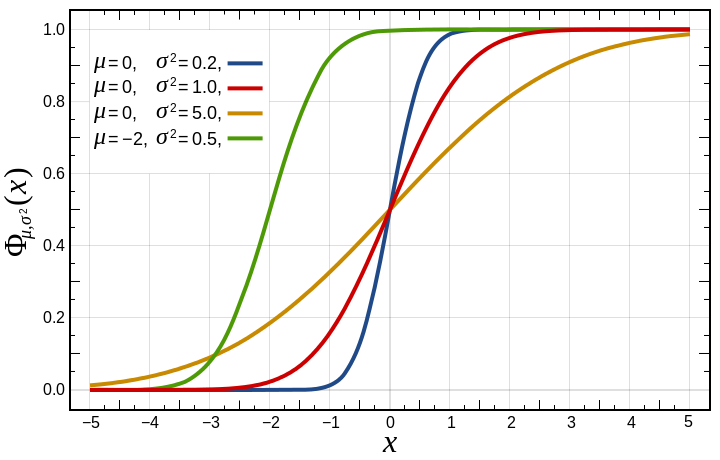
\includegraphics[width=5.5cm]{pic/gauss_density}}
\subfigure[Cumulative distribution function] {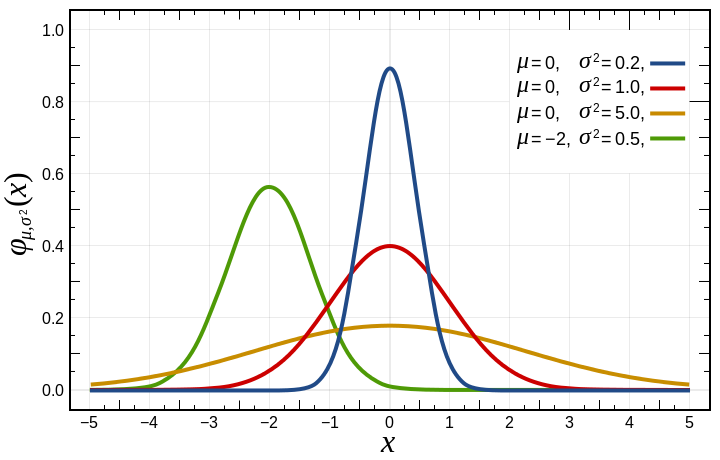
\includegraphics[width=5.5cm]{pic/gauss_cumul}} 
}
\caption{\label{gauss} 
Gaussian distribution 
} 
\centerline{
\subfigure[Probability density function] {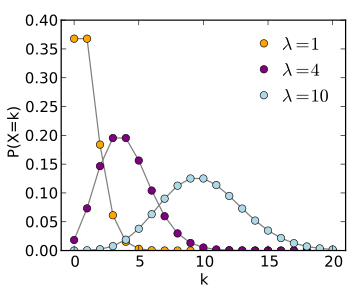
\includegraphics[width=5.5cm]{pic/Poisson_pmf}}
\subfigure[Cumulative distribution function] {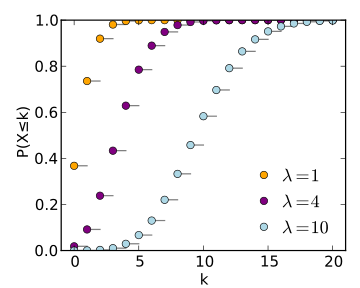
\includegraphics[width=5.5cm]{pic/Poisson_cdf}} 
}
\caption{\label{poisson} 
Poisson distribution 
}
\centerline{
\subfigure[Probability density function] {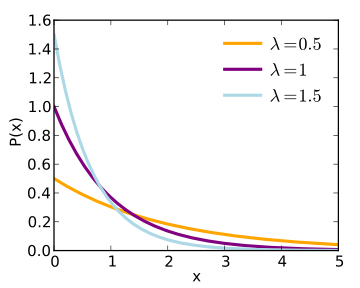
\includegraphics[width=5.5cm]{pic/exp_pmf}}
\subfigure[Cumulative distribution function] {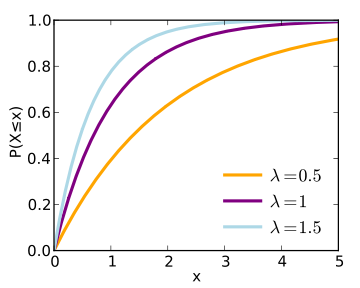
\includegraphics[width=5.5cm]{pic/exp_cdf}} 
}
\caption{\label{exp} 
Exponential distribution 
} 
\centerline{
\subfigure[Probability density function] {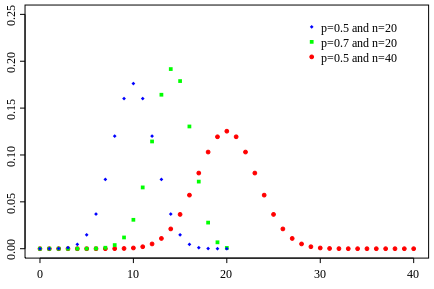
\includegraphics[width=5.5cm]{pic/binomial_pmf}}
\subfigure[Cumulative distribution function] {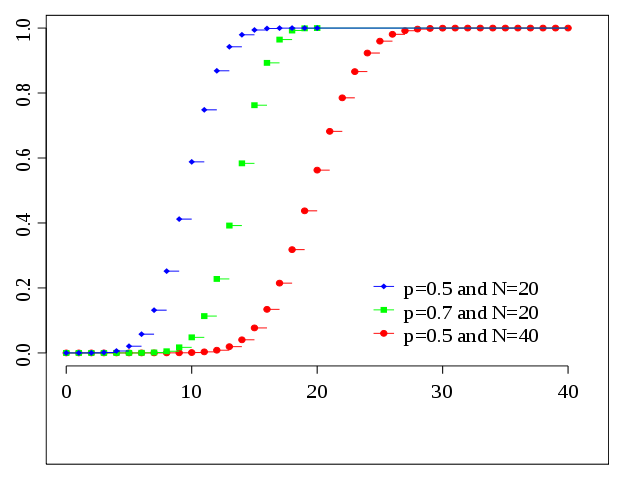
\includegraphics[width=5.5cm]{pic/binomial_cdf}} 
}
\caption{\label{binomial} 
Binomial distribution 
} 
\end{figure}



% ================ Measurement ==============
\subsection{Measurement on Samples}

In practice, we (almost) never analyse the entire population. We always work on a subset of it called \textbf{sample}. The \textbf{variance} is the variation between elements of our sample, that we hope to be the same as the population. The \textbf{biais} is the systematic variation between the entire population and the sample we chose.

When randomly select elements of the population to be part of the sample, we have a great chance that the biais is small (i.e. that the distribution of the sample correspond to the distribution of the population). But do not forget that there is a probability (even if a small one) to select elements that \textbf{biased our measures}! This probability can even increase when you clean the data, if you don't do it wisely.

A stupid example could be a study on population education in which, during the cleaning, you remove the answers containing misspelling. Uneducated people are more likely to commit misspelling so, removing them, you artificially biais the sample.

% ================ Test Statistic ==============
\subsection{Test Statistic}

(The only good and easy-to-understand explanation about test statistic I ever found is available on \href{http://hamelg.blogspot.ch/2015/11/python-for-data-analysis-part-24.html?view=flipcard}{hamelg.blogspot})

The idea behind test statistic is \textbf{instead of proving that our assumption is true, let's calculate the probability that our observations occur by chance. If this probability is very low, then there is a good chance that our hypothethis is true!}

The probability that this happen by chance is called \textbf{null hypothesis} $H_0$. The hypothesis we made is $H_A$.

% ================ Test Statistic ==============
\subsubsection{Example with t-test}

Let's take the example on FIG \ref{pic:ttest}. The \textbf{Null Hypthesis} $H_0$ represents the distribution of observation we can do, assuming there is no correlation between the values we measured. The \textbf{Alternative} is $H_A$, our hypothesis which states that, at the opposite, their is correlations.
\begin{itemize}
	\item If the observation we test is $x=3$, there is \textbf{less than 5\% probabilities that it was produced by $H_0$} ($pvalue \leq 0.5$). Our hypothesis $H_A$ is considered true.

	\item If the observation we test is $x=0$, there is \textbf{more than 5\% probabilities that it was produced by $H_0$} (more or less 40\%). Our hypothesis $H_A$ is considered false.
\end{itemize}

{\color{red} An important thing to notice is that \textbf{it does not provide truth on statistic}, it only provides information about how likely is the null hypothesis! Let's look back to the example}

\begin{itemize}
	\item The $x=3$ observation \textbf{could have been produced by the red area}, meaning that it's part of the small 5\% chance of being produced by the $H_0$. The test will say that our hypthesis is true, which will be a \textbf{false positiv}.

	\item The $x=0$ observation \textbf{could have been produced by the blue area}, meaning that even it $H_0$ have great chance to produce it, it's was in fact produced by $H_A$.  The test will say that our hypthesis is false, which will be a \textbf{false negativ}.
\end{itemize}

\begin{figure}[h]%---------------FIG--------------
 \centering
 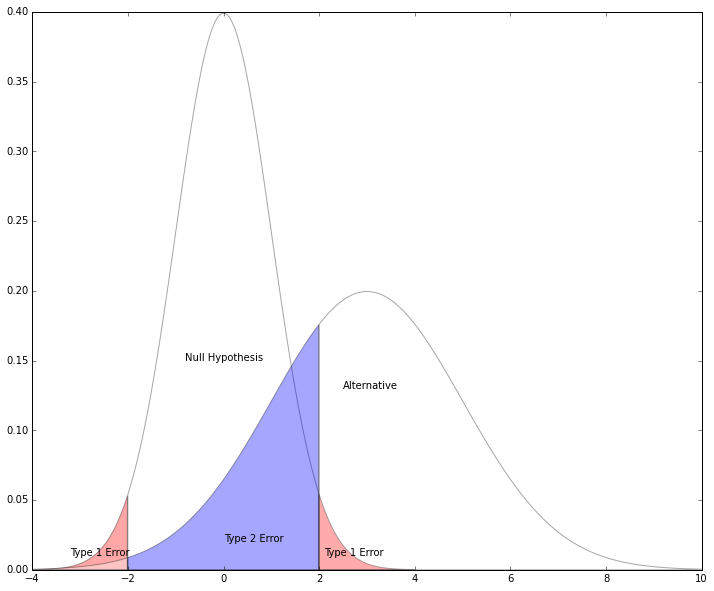
\includegraphics[width=10cm]{./pic/t-test}
 \caption{\label{pic:ttest} T-Test example}
\end{figure}

% ================ Test Statistic ==============
\subsubsection{Choose the right test}

A lot of test exists and we must choose wisely which one to use, according with data and hypothesis characteristics. FIG \ref{pic:testtree} show a decision tree helping to choose the test which suits best our situation.

\begin{itemize}
 \item Question ? 
 \item Data type ?
 \item Sample size
 \item Variance known? 
 \item Variance of several groups equals?
 \item ...
\end{itemize}

\begin{figure}[h]%---------------FIG--------------
 \centering
 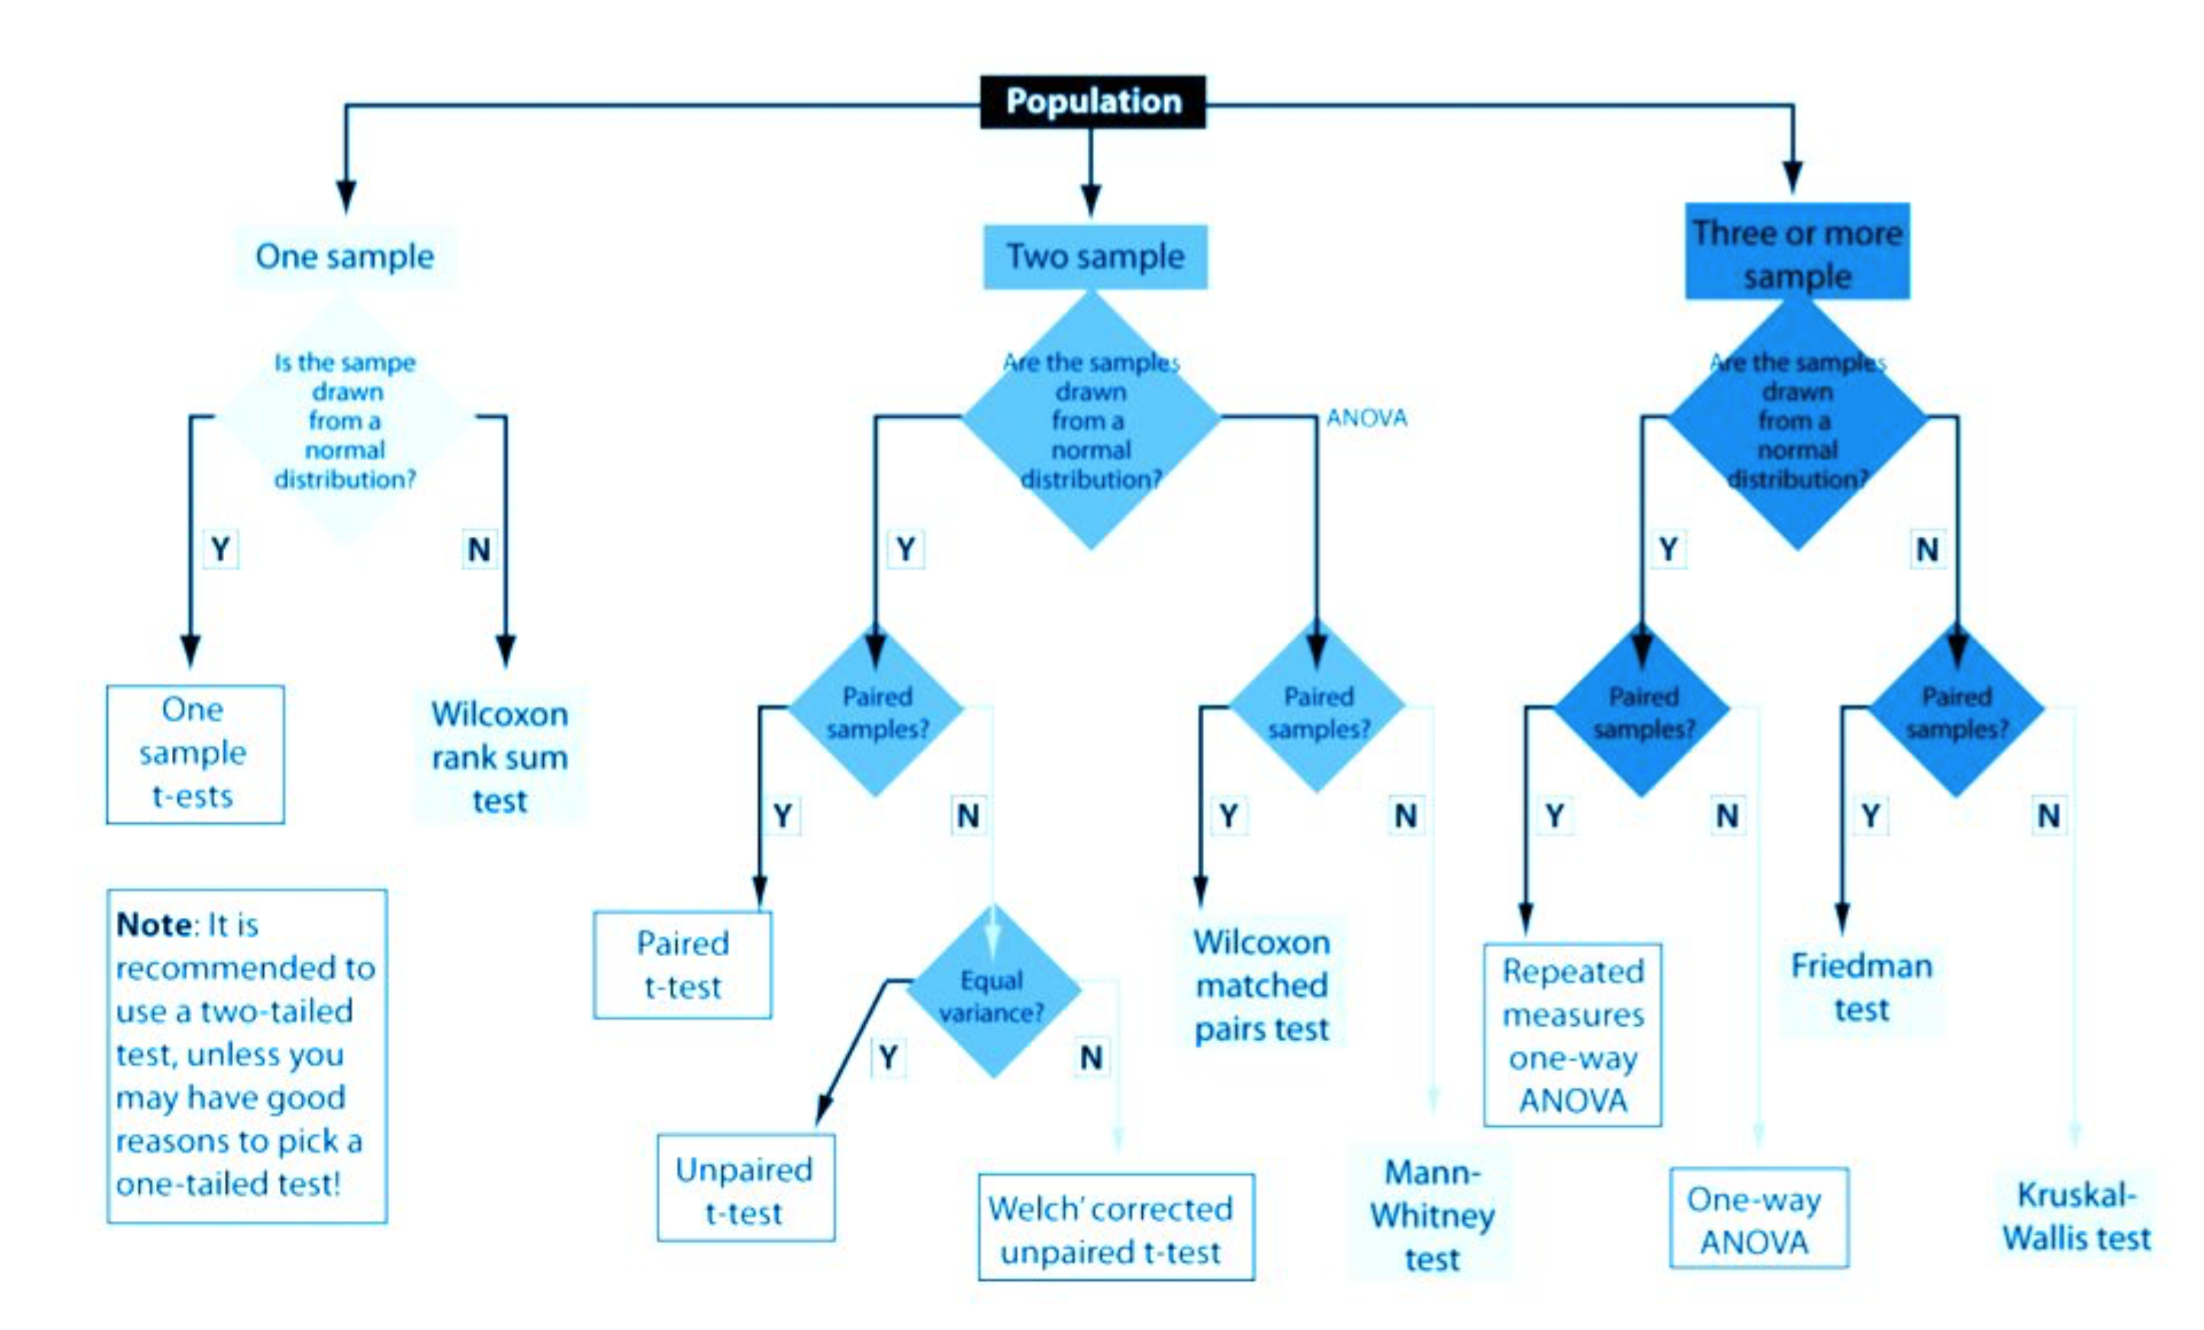
\includegraphics[width=15cm]{./pic/choose_test}
 \caption{\label{pic:testtree} Statistical test descision tree}
\end{figure}




Multiple Hypothese Testing: \\
If you perform experiments over and over, you're bound to find something. Significance level must be adjusted down when performing multiple hypothesis tests. 
\\\\
Familywise Error Rate: \\
Error rate when too many experiments are done.. Je te laisse developer =P. There are some corrections: Bonferroni and Sidak.
\\\\
Non-Parametric Tests: \\
All the tests so fare assume that the data are {\bf normally distributed} and that the samples are {\bf independent of each other and all have the same distribution.} (IID) They may be innacurate if those assumptions are not met. Therefore, make sure the data satisfies the assumptions of the test we're using. Watch out for:
\begin{description}
 \item[Outliers] will corrupt many tests that use variance estimates.
 \item[Correlated values as samples], e.g. if you repeated measurements on the same subjective
 \item[Skewed (bias) distributions] give invalid results.
\end{description}
K-S test: \\
K-S (Kolmogorov-Smirnov) test is a very useful test for checking whether two (continuous or discrete) distributions are the same. 
\begin{itemize}
 \item In the {\bf one-sided test}, an observed distribution (e.g. some observed values or a histrogram) is compared against a reference distribution (e.g., power-law).
 \item In the {\bf two-sided test}, two observed distrubtions are compared.
 \item The K-S statistic is just the {\bf max distance between the CDFs} (Cumulative Distribution Function) of the two distributions.
 \item The K-S test can be used to test {\bf whether a data sample has  anormal distribution} or not.
 \item Thus it can be used as a sanity check for any common parametric test (which assumes normally-distributed data).
 \item It can also be used to compared distributions of data values in large data pipeline: {\bf Most errors will distort the distribution of a data parameter and a K-S test can detect this.}
\end{itemize}
This test is expensive! 
\\
{\bf WE NEED TO ADD MORE STUFF ON THE K-S TEST. CHECK ON WIKIPEDIA.. =) }
   






%======= TABLEAU ===========
%\begin{center} %---------------Tab--------------
%\begin{tabular} {| c | c | c | c | c | c |}
%\hline
 %& & & & & $\\ \hline
%\end{tabular}
%\end{center}


%===========GRAPH================
%\begin{figure} %---------------------Graph---------------------------
%\begin{center}
%\includegraphics[width=12cm]{graph/ampli2} 
%\end{center}
%\caption{\em  \label{label}
%L�gende
%}
%\end{figure}


%========SUBGRAPH=======
%\begin{figure} [h] %----------- SubGraph ---------------------
%\centerline{
%\subfigure[ sublegend ] {\label{sfig:thetat} \includegraphics[width=7cm]{ graph/graph_convdt3 } }
%\subfigure[ sublegend ] {\label{sfig:thetafin} \includegraphics[width=7cm]{ graph/graph_convtfin } } 
%}
%\caption{\label{ label } 
%L�gende
%} 
%\end{figure}








\end{document} %%%% THE END %%%%
